\documentclass[12pt]{article}
\usepackage[letterpaper,left=2.25cm,top=3.0cm,right=2.25cm,bottom=2.0cm, headsep=1.5cm]{geometry}
\usepackage{fancyhdr}
\usepackage[utf8]{inputenc}
\usepackage[T1]{fontenc}
\usepackage[spanish,mexico]{babel}
%\usepackage[letterpaper,margin=2.5cm]{geometry}
\usepackage{setspace}
\usepackage{titlesec}
\usepackage{tocloft}
\usepackage{graphicx}
\usepackage{array}
\usepackage{longtable}
\usepackage{float}
\newcolumntype{C}[1]{>{\centering\arraybackslash}p{#1}} % Centrar 

%\usepackage{hyperref}
\usepackage{wallpaper}
% Para utilizar el formato de citas IEEE y comentar los dos parrafos siguientes. Ademas de utilizar el comando \cite en vez de \cite
\usepackage[backend=biber,sorting=none]{biblatex}
% Para utilizar el formato APA, sugiero comentar la linea anterior y descomentar las dos proximas lineas. Ademas de utilizar el comando \cite en vez de \cite
%\usepackage[backend=biber,style=apa]{biblatex}
%\DeclareLanguageMapping{english}{american-apa}

\makeatletter
\DefineBibliographyExtras{spanish}{%
  \setcounter{smartand}{1}%
  \let\lbx@finalnamedelim=\lbx@es@smartand
  \let\lbx@finallistdelim=\lbx@es@smartand
}
\renewbibmacro*{name:delim:apa:family-given}[1]{%
  \ifnumgreater{\value{listcount}}{\value{liststart}}
    {\ifboolexpr{
       test {\ifnumless{\value{listcount}}{\value{liststop}}}
       or
       test \ifmorenames
     }
       {\printdelim{multinamedelim}}
       {\lbx@finalnamedelim{#1}}}
    {}}
\makeatother
% Estas lineas permiten romper los hipervinculos muy largos en las referencias!!!!
\setcounter{biburllcpenalty}{7000}
\setcounter{biburlucpenalty}{8000}
\addbibresource{Referencias.bib} % ARCHIVO DE BIBLIOGRAFÍA


\usepackage[bookmarks=true,breaklinks=true,bookmarksopen=false,colorlinks=true,linkcolor=blue]{hyperref}
\usepackage[hyphenbreaks]{breakurl}
\usepackage{pdfpages} % Incluir PDF en documento en LATEX
\setstretch{1.3}

\usepackage{soul}


% CONSTANTES NECESARIAS PARA EL DOCUMENTO ---> MODIFIQUEN A SU CRITERIO
\newcommand{\NombreAlumno}{David Alejandro Ibarra Castañeda}
\soulregister{\NombreAlumno}{1}
% NUNCA PONGAN EL TITULO EN MAYUSCULAS!!
\newcommand{\NombreProyecto}{Plataforma integral de Atención Unificada y Registro Automatizado para la Agencia de Innovación e Inteligencia Digital de Tamaulipas} 
% Noten los \\ para insertar un ENTER del texto en el encabezado. NUNCA PONGAN EL TITULO EN MAYUSCULAS!!
\newcommand{\NombreProyectoheader}{Plataforma integral de Atención Unificada y Registro Automatizado para la Agencia de Innovación e Inteligencia Digital de Tamaulipas}
\newcommand{\NombreTSU}{Desarrollo de Software Multiplataforma}
\newcommand{\UnidadEconomica}{Agencia de Innovación e Inteligencia Digital de Tamaulipas}
\newcommand{\nasesorempresaria}   {Ing. David Angel Gallardo Soto}
\newcommand{\nasesorinstitucional}{Dr. Marco Aurelio Nuño-Maganda}
\newcommand{\Matricula}           {2430249}  %SU MATRICULA
\newcommand{\ncuatrimestre}{Mayo-Agosto 2026}
% ESTA ES LA FECHA EN LA QUE EL ASESOR INSTITUCIONA EVALUA EL INFORME
\newcommand{\fechaAutorizacionInforme}               {31 de Julio de 2026} 
% ESTA ES LA FECHA EN LA QUE EL ASESOR INSTITUCIONA PROGRAMA LA EXPOSCION 
\newcommand{\DiaEvaluacionPesentacion}{12}
\newcommand{\MesEvaluacionPesentacion}{Agosto}
\newcommand{\AnhoEvaluacionPesentacion}{2026}
\newcommand{\fechaPortada}               {\MesEvaluacionPesentacion~de~\AnhoEvaluacionPesentacion}
\newcommand{\HoraEvaluacionPesentacion}{10:00 hrs}

\newcommand{\modalidadEvaluacionPesentacion}{Presencial} % Otras opciones: Virtual
\newcommand{\tipoAulaOficinaEnlacePesentacion}{la Oficina} % Otras opciones: la oficia/el aula/enlace
\newcommand{\AulaEvaluacionOEnlaceMeetPesentacion}{I-XXX69} %otras opciones: si es un elance de meet, rodearlo \url{}

%\newcommand{\modalidadEvaluacionPesentacion}{Virtual} % Otras opciones: Virtual
%\newcommand{\tipoAulaOficinaEnlacePesentacion}{el enlace} % Otras opciones: la oficia/el aula/el enlace
%\newcommand{\AulaEvaluacionOEnlaceMeetPesentacion}{\url{http://www.upvictoria.edu.mx}} %otras opciones: si es un elance de meet, rodearlo \url{}

\newcommand{\ncarrera}            {Ingeniería en Tecnologías de la Información e Innovación Digital}


\fancyhead{} % Clear all header fields
\fancyhead[C]{%
    \begin{tabular}{@{} m{0.2\textwidth} m{0.5\textwidth} m{0.2\textwidth} @{}}
        % Left image
        
\includegraphics[height=1.20cm]{UTYP.png}
        &
        % Center text (multiline, centered)
        \centering
        \scriptsize{\NombreProyectoheader}
        %\textbf{University Name} \\ 
        %Department of Something \\ 
        %Course Title
        &
        % Right image
        %\raggedleft
        
\includegraphics[height=1.5cm]{LogoUPV_2023.png}
    \end{tabular}
}


%\usepackage{imakeidx}
%\makeindex[title=New Index Title]

%\renewcommand{\contentsname}{Whatever}
%

%\usepackage[english]{babel}

\addto\captionsspanish{% Replace "english" with the language you use
  \renewcommand{\contentsname}%
    {Contenido temático}%
}


\renewcommand\spanishtablename{Tabla}

\begin{document}

% PAGINA 1 - PORTADA
\setcounter{page}{0}
\pagenumbering{roman}
\thispagestyle{empty}




\begin{titlepage}


\vspace*{-2cm}
\begin{center}
\begin{tabular}{cp{6cm}c}

\includegraphics[height=2.25cm]{UTYP.png} & 
& 
\includegraphics[height=2.25cm]{LogoUPV_2023.png}   \\
\end{tabular} \\[0.5cm]



{\Large \textbf{UNIVERSIDAD POLITÉCNICA DE VICTORIA}}\\[1.0cm]

{\Large \textbf{REPORTE DE ACTIVIDADES DEL PROYECTO}}\\[0.75cm]

{\Large \MakeUppercase{\NombreProyecto}}\\[1.0cm]

QUE PRESENTA

\textbf{\MakeUppercase{\NombreAlumno}}\\[1.0cm]

EN CUMPLIMIENTO DE LA ESTADÍA TSU EN\\
\textbf{\MakeUppercase{\NombreTSU}}\\[0.75cm]

ASESOR INSTITUCIONAL\\
\textbf{\MakeUppercase{\nasesorinstitucional}}\\[0.5cm]

UNIDAD ECONÓMICA RECEPTORA:\\
\textbf{\MakeUppercase{\UnidadEconomica}}\\[0.5cm]

ASESOR DE LA UNIDAD ECONÓMICA\\
\textbf{\MakeUppercase{\nasesorempresaria}}\\[0.5cm]


\end{center}
\begin{flushright}
Ciudad Victoria, Tamaulipas, \fechaPortada.
\end{flushright}

\end{titlepage}


\newpage
% PAGINA 1 - PORTADA
\setcounter{page}{0}
\pagenumbering{roman}
\pagestyle{empty}
\ULCornerWallPaper{1}{Membrete2023.pdf}
\vspace*{2cm}


% Pagina de la autorizacion para exponer
\begin{center}
{\Large \textbf{Formato de autorización para exposición de Estadía de}}\\[0.125cm]
{\Large \textbf{Técnico Superior Universitario}}\\[0.25cm]
\end{center}

\noindent
Fecha y lugar en que se emite: \textbf{Ciudad Victoria, Tamaulipas, a \fechaAutorizacionInforme } \\[0.125cm]
Nombre completo del estudiante: \textbf{\NombreAlumno} \\[0.125cm]
Matrícula: \textbf{\Matricula}  \\[0.125cm]
Programa Académico: \textbf{\ncarrera}  \\[0.25cm]

\noindent
Por medio del presente, se le informa que tras realizar su Estadía en la empresa \textbf{\UnidadEconomica} llevando a cabo el proyecto: \textbf{\NombreProyecto}, durante el periodo comprendido \textbf{\ncuatrimestre} logrando una ponderación de \_\_\_\_  (60\% posibles) para el criterio de reporte; por lo tanto, se otorga la oportunidad de exponer el trabajo realizado por medio de un informe ejecutivo programado para el día \textbf{\DiaEvaluacionPesentacion} del mes de \textbf{\MesEvaluacionPesentacion} del año en curso en un horario de \textbf{\HoraEvaluacionPesentacion} en modalidad \textbf{\modalidadEvaluacionPesentacion} en \textbf{\tipoAulaOficinaEnlacePesentacion} \textbf{\AulaEvaluacionOEnlaceMeetPesentacion}.

\vspace{0.25cm}

\noindent
Sin otro particular, se le recomienda estar disponible para iniciar su exposición 10 minutos antes de la indicación oficial.

\vspace{0.5cm}

\begin{center}
\begin{tabular}{p{10cm}}
\multicolumn{1}{c}{Atentamente}   \\
 \\
 \\ \hline
\multicolumn{1}{c}{\nasesorinstitucional}   \\
\multicolumn{1}{c}{Asesor institucional}   \\
\end{tabular}
\end{center}

\clearpage
\ULCornerWallPaper{1}{Membrete2023.pdf}

\vspace*{3cm}



\begin{center}
{\large \textbf{Control sumativo de Estadía para Técnico Superior Universitario}}
\end{center}

\vspace{0.5cm}

\begin{center}
\begin{tabular}{|p{6cm}|C{4cm}|C{4cm}|}
\hline
\textbf{Criterio} & \textbf{Valor / Ponderación} & \textbf{Calificación} \\ \hline
Reporte & 60\% & \\ \hline
Exposición & 40\% & \\ \hline
Calificación final & \multicolumn{2}{c|}{ } \\ \hline
\end{tabular}
\end{center}

\vspace{0.8cm}

%\noindent
%\textbf{Nota:} para completar este documento deberá sustentar su decisión con base en las rúbricas oficiales de la institución diseñadas para cada evaluación.

\begin{center}
\begin{tabular}{|p{10cm}|}
\hline
\multicolumn{1}{|c|}{\textbf{Datos de la evaluación sumativa}}\\
\multicolumn{1}{|c|}{Fecha: \textbf{\DiaEvaluacionPesentacion}  / \textbf{\MesEvaluacionPesentacion} / \textbf{\AnhoEvaluacionPesentacion}} \\ \hline
%\multicolumn{1}{c}{Atentamente}   \\
 \\
 \\ \hline
\multicolumn{1}{c}{\nasesorinstitucional}   \\
\multicolumn{1}{c}{Asesor institucional}   \\
\end{tabular}
\end{center}





%\vspace{1cm}

%\noindent




%\vspace{1.5cm}

%\noindent
%Firma: \hrulefill

%\vspace{1cm}

%\noindent
%Nombre del Asesor institucional: \nasesorinstitucional \hrulefill


\clearpage
\ClearWallPaper
\thispagestyle{fancy}
\addcontentsline{toc}{section}{Resumen}
%\vspace*{1cm}
\section*{Resumen}




\clearpage
\thispagestyle{fancy}
\addcontentsline{toc}{section}{Abstract}
%\vspace*{1cm}
\section*{Abstract}


\clearpage
%\renewcommand{\indexname}{Contenido temático}

\thispagestyle{empty}
\ClearWallPaper
\tableofcontents


%\chapter{Introducción}

\clearpage
\pagenumbering{arabic}
\setcounter{page}{1}
\pagestyle{fancy}

\section{Introducción}
El reporte que usted está leyendo es el resultado de todo lo que he realizado en mis estadías TSU, dentro de la Agencia de Innovación e Inteligencia Digital de Tamaulipas... una empresa que se dedica a diseñar estrategias digitales, desarrollar plataformas tecnológicas, mejorar la experiencia ciudadana en trámites y servicios, en la modernización de la infraestructura digital, así como el fomento de una cultura de datos abiertos, transparencia e innovación. El sistema que he planteado tiene como propósito ayudar al personal de la agencia a registrar a los visitantes, llamadas y agendar salas sin la necesidad de andar gastando papel y pluma... pudiendo realizar los tramites de manera digital y sin gastar recursos físicos. Este proyecto no solamente automatiza y optimiza el flujo de trabajo de la Agencia, sino que fomenta la seguridad digital y la privacidad de los trabajadores.

%\chapter{Descripción de la Unidad Económica}



\clearpage
\section{Descripción de la Unidad Económica}

\subsection{Giro}
La Agencia de Innovación e Inteligencia Digital de Tamaulipas pertenece al sector de servicios, es decir, se dedican a desarrollar software y plataformas para la automatización de tareas cotidianas de los trabajadores y para brindar un mejor servicio a los visitantes del lugar.


\subsection{Descripción General}
La agencia ha destacado por la capacidad de manejar múltiples tramites a la vez, a través de herramientas desarrolladas por ellos mismos para así poder dividirse toda la carga de trabajo entre los integrantes. El departamento busca  soluciones que puedan resumir y optimizar los procesos de trabajo, a través de servicios simplificados.


\subsection{Departamento de trabajo}
El área en el que me encontré trabajando se llama "Departamento de Digitalización de Tramites y servicios Simplificados". Como su nombre lo indica, el rol de esa área consiste en desarrollar softwares que permitan agilizar y automatizar los trámites para así ahorrar tiempo y esfuerzo... como por ejemplo mejorar el seguimiento de los visitantes, la generación de reportes mas rápidos, facilitar la comunicación entre recepción y administración, etc. También son los responsables de coordinar, implementar y supervisar en Tamaulipas las políticas, estrategias y modelos nacionales de simplificación administrativa y transformación digital previstos en la Ley Nacional \cite{departamentoDeDigitalizacionyAutomatizacionDeTramites:agencia}.


En la agencia, hay un director que se encarga de gestionar y supervisar todos los departamentos que existen en el lugar, el cual se llama David Angel Gallardo Soto (mi asesor empresarial) y cada departamento tiene a su respectivo jefe, por lo que la agencia cuenta con subáreas con sus sub-directores.

Debido a que el director suele estar muy ocupado debido a que es el mero jefe de toda la agencia, contaba con un titular, quien se encargaba de supervisarme y de guiarme en el proyecto. Los titulares son los jefes de los diferentes departamentos que existen y en mi caso, tenia que acudir primero con el antes de ir con mi asesor empresarial. En la figura \ref{fig:mapaDelPiso}, se muestra el mapa de la agencia, desde sus cubículos, hasta los baños.

\begin{figure}[H]
    \centering
    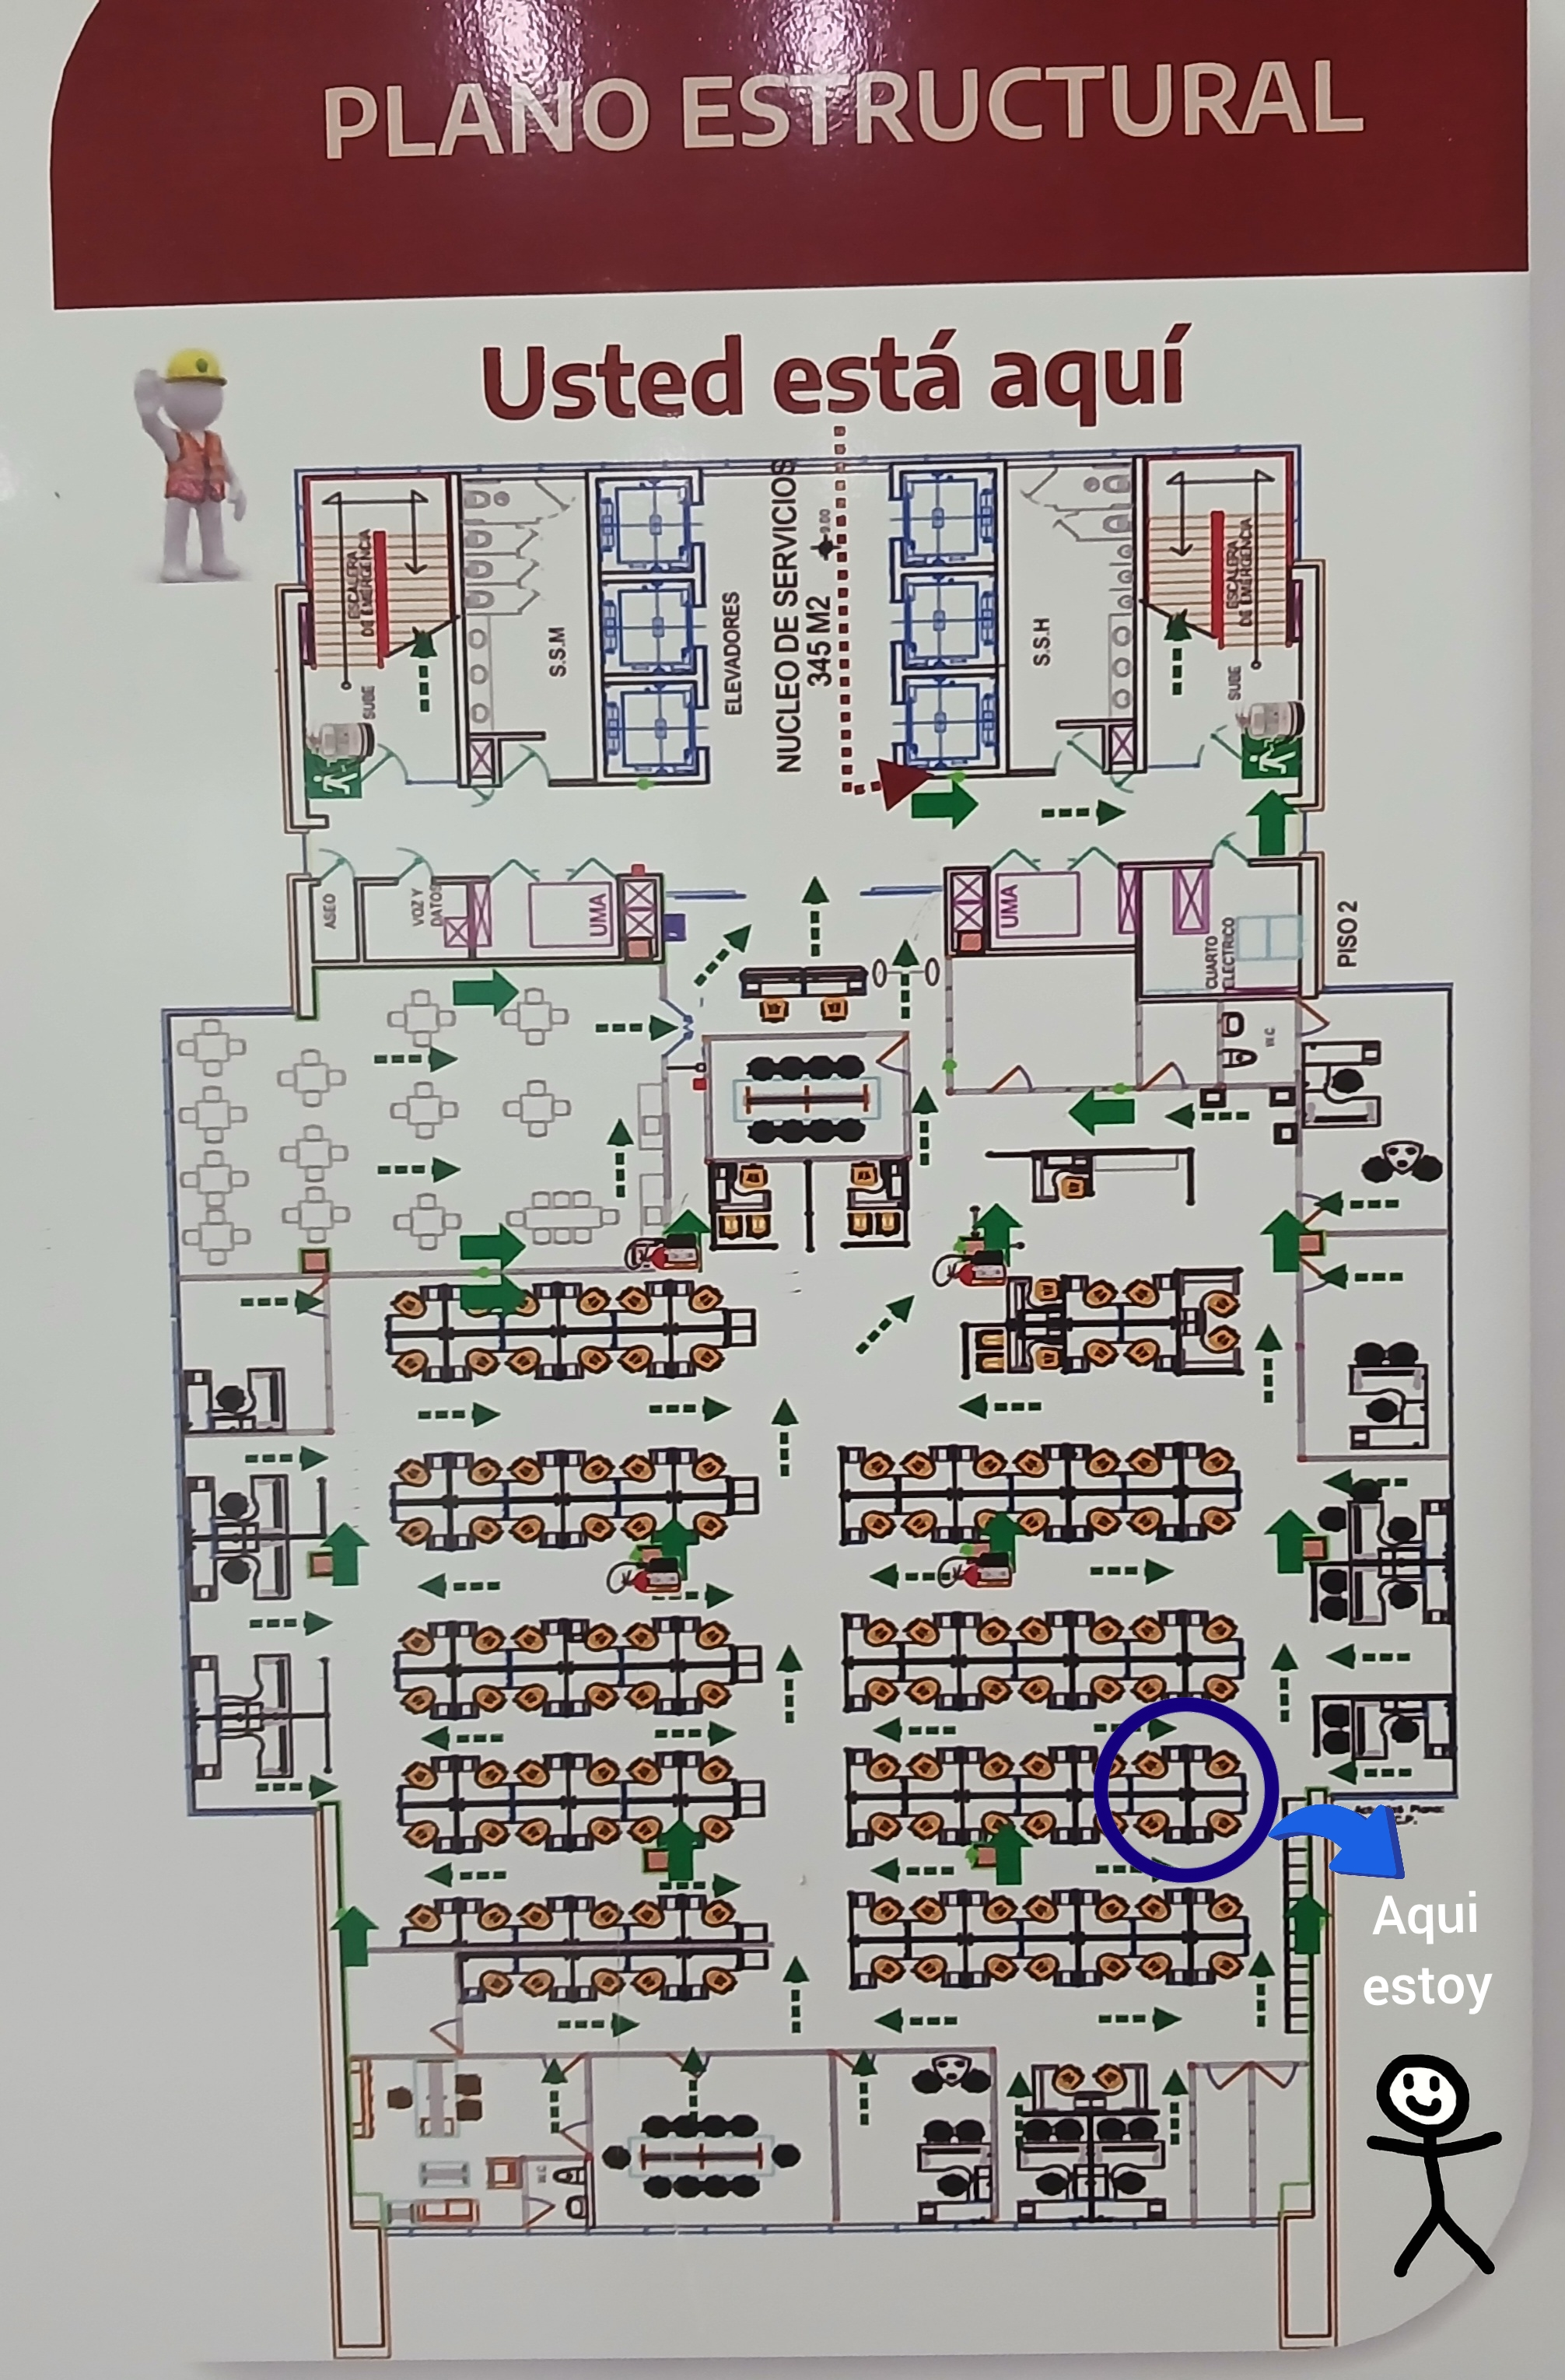
\includegraphics[width=0.8\linewidth]{figs/MapaDelPiso.jpg}
    \caption{Mapa de toda la Agencia de Innovación e Inteligencia Digital de Tamaulipas. \cite{AIIDT:Ubicacion}}
    \label{fig:mapaDelPiso}
\end{figure}

\subsection{Misión}
Gestionar y coordinar las acciones institucionales de dependencias y entidades de la administración pública mediante procesos administrativos orientados al otorgamiento de resultados y rendición de cuentas, que aseguren la planeación y ejecución de políticas públicas orientadas a la transformación y desarrollo del Estado de Tamaulipas para lograr el bienestar social y económico sostenible de las familias Tamaulipecas.

\subsection{Visión}
Las dependencias y entidades de la administración pública respondan a las necesidades y expectativas de bienestar y desarrollo, mediante programas y proyectos basados en políticas públicas planificadas en un contexto de mediano y largo plazo, en un diálogo permanente entre sociedad y Gobierno.

\subsection{Infraestructura}
\subsubsection{A nivel físico o de Hardware}
La agencia cuenta con equipos de cómputo, repetidores de red en el techo para ampliar la señal del wifi y por supuesto, la empresa posee una sala para los servidores locales, por lo que la organización cuenta con una red propia para los trabajadores. También tienen una red para los visitantes y esta es gratuita.



\subsubsection{A nivel de Software}
Las herramientas que utilizan para desarrollar softwares y plataformas son: Laravel 13, Python con FastAPI, PostgreSQL para las bases de datos, git con Github y Docker para el manejo de contenedores.


\subsection{Ubicación}
Piso 2, Torre Nueva

\clearpage
%\chapter{Objetivos Operativos}
\section{Objetivos Operativos}

\begin{enumerate}
    \item Analizar los procesos actuales del área de recepción mediante reuniones con el asesor empresarial y el uso de técnicas de recolección de datos, con la finalidad de estructurar los requerimientos técnicos y funcionales del sistema.
    \item Diseñar la arquitectura lógica de la plataforma y el modelo de datos relacional a través del modelado de diagramas UML en la herramienta PlantUML, asegurando una estructura escalable para la gestión unificada de visitantes y salas.
    \item Construir la lógica de negocio y los servicios web (APIs) en el backend mediante el uso del framework Laravel 13, garantizando la automatización de las llamadas y el correcto procesamiento de los registros de entrada.
    \item Desarrollar las interfaces gráficas de usuario utilizando las plantillas de diseño institucionales proporcionadas por la propia empresa, facilitando una interacción intuitiva del personal con los módulos de atención del sistema.
    \item Integrar los algoritmos de identificación biométrica en la plataforma mediante la configuración de librerías de visión artificial y scripts de captura de video, permitiendo el correcto reconocimiento facial de los usuarios en tiempo real.
    \item Ejecutar pruebas de rendimiento, seguridad y consistencia localmente dentro de entornos contenedorizados con Docker, permitiendo la detección, depuración y corrección oportuna de fallos en los módulos inteligentes antes de su producción.
    \item Elaborar la documentación técnica del sistema, los diccionarios de datos y los manuales de usuario mediante procesadores de texto y estándares de ingeniería de software, garantizando la correcta operación, transferencia y mantenimiento futuro de la plataforma.
\end{enumerate}
\subsection{Objetivo General}
Desarrollar una plataforma que permita optimizar los procesos de registro y seguimiento de los visitantes en la Agencia de Innovación e Inteligencia Digital de Tamaulipas, mediante tecnologías de reconocimiento facial que fortalezcan la seguridad y la eficiencia operativa de la institución.

\subsection{Objetivos Específicos}
\begin{enumerate}
    \item Analizar los procesos actuales de recepción para determinar los requerimientos funcionales y técnicos del sistema.
    \item Diseñar la arquitectura de software y el modelo de datos que den soporte a la gestión unificada de visitantes y salas.
    \item Construir la lógica de negocio en el backend para la administración automatizada de llamadas y registros de entrada.
    \item Desarrollar interfaces de usuario intuitivas que faciliten la interacción del personal con los módulos de atención del sistema.
    \item Integrar algoritmos de identificación biométrica para la captura y reconocimiento facial de los usuarios.
    \item Ejecutar pruebas de rendimiento y seguridad para validar el correcto funcionamiento de los módulos inteligentes.
    \item Elaborar la documentación técnica y manuales de usuario que garanticen la correcta operación y mantenimiento futuro del sistema.
\end{enumerate}



%\chapter{Metodología}
\clearpage
\section{Metodología}
Durante el transcurso de mis estadías TSU, me gustaría comentar que el desarrollo de mi proyecto, al igual que mi entorno de trabajo, se puso a marcha desde mi propio celular... si, leyó bien, mi proyecto se realizo en un Android 16 utilizando Termux como emulador de terminal (instalado desde F-Droid). La plataforma que desarrolle utiliza el siguiente stack de tecnologías:  Laravel 13, php 8.5, postgreSQL 18.2 con la extensión de pgvector, FusionAuth con OIDC, nodejs-lts y por ultimo, la herramienta con la que he estado trabajando todas estas tecnologías: Termux.

\subsection{Análisis de requerimientos y especificación del sistema}

En la primera semana de las estadías TSU, mi tutor me entrevistaba en su cubículo para determinar las tecnologías y metodologías a utilizar para el desarrollo de mi proyecto y en la forma de trabajar dentro de la agencia. 

En la tercera semana de las estadías, mi tutor me convocó a una reunión a las 3:00 p.m, en donde un profesional me mostraría a detalle un repositorio de Github, que contendría una plantilla que realizaron ellos mismos para utilizarla en mi proyecto, es decir, una plantilla para proyectos de Laravel 13. El profesional me explico acerca de la "modularización en Laravel", que en resumen es como si tuviéramos mini Laravels dentro de un proyecto de Laravel y de hecho, la plantilla utiliza módulos para separar toda la lógica de negocio \cite{medium:inicio}.

Durante la reunión, me explicaron que todo el equipo de la agencia utiliza \textit{FusionAuth} en sus proyectos de Laravel... para la autenticación y validación de los usuarios a la hora de navegar en las vistas de Laravel \cite{AIIDT:Documentacion}.

Durante esta semana, empece a definir los requisitos funcionales y no funcionales del proyecto.

\subsection{Diseño de la arquitectura y modelado de datos}

Entre la primera y tercera semana de las estadías, empecé a realizar los primeros diseños del sistema, como el diagrama de flujo de la plataforma y algunos Wireframes de baja fidelidad del proyecto.

En la figura \ref{fig:DiagramaDeFlujoBasico}, tenemos el diagrama de flujo del proyecto. A simple vista se ve muy básico, sin embargo, este diseño fue hecho a mano como diseño de prueba. Mas adelante veremos el verdadero diagrama de flujo.

%%Le volvemos a agregar el formato !tbh a las imagenes


\begin{figure}[H]
    \centering
    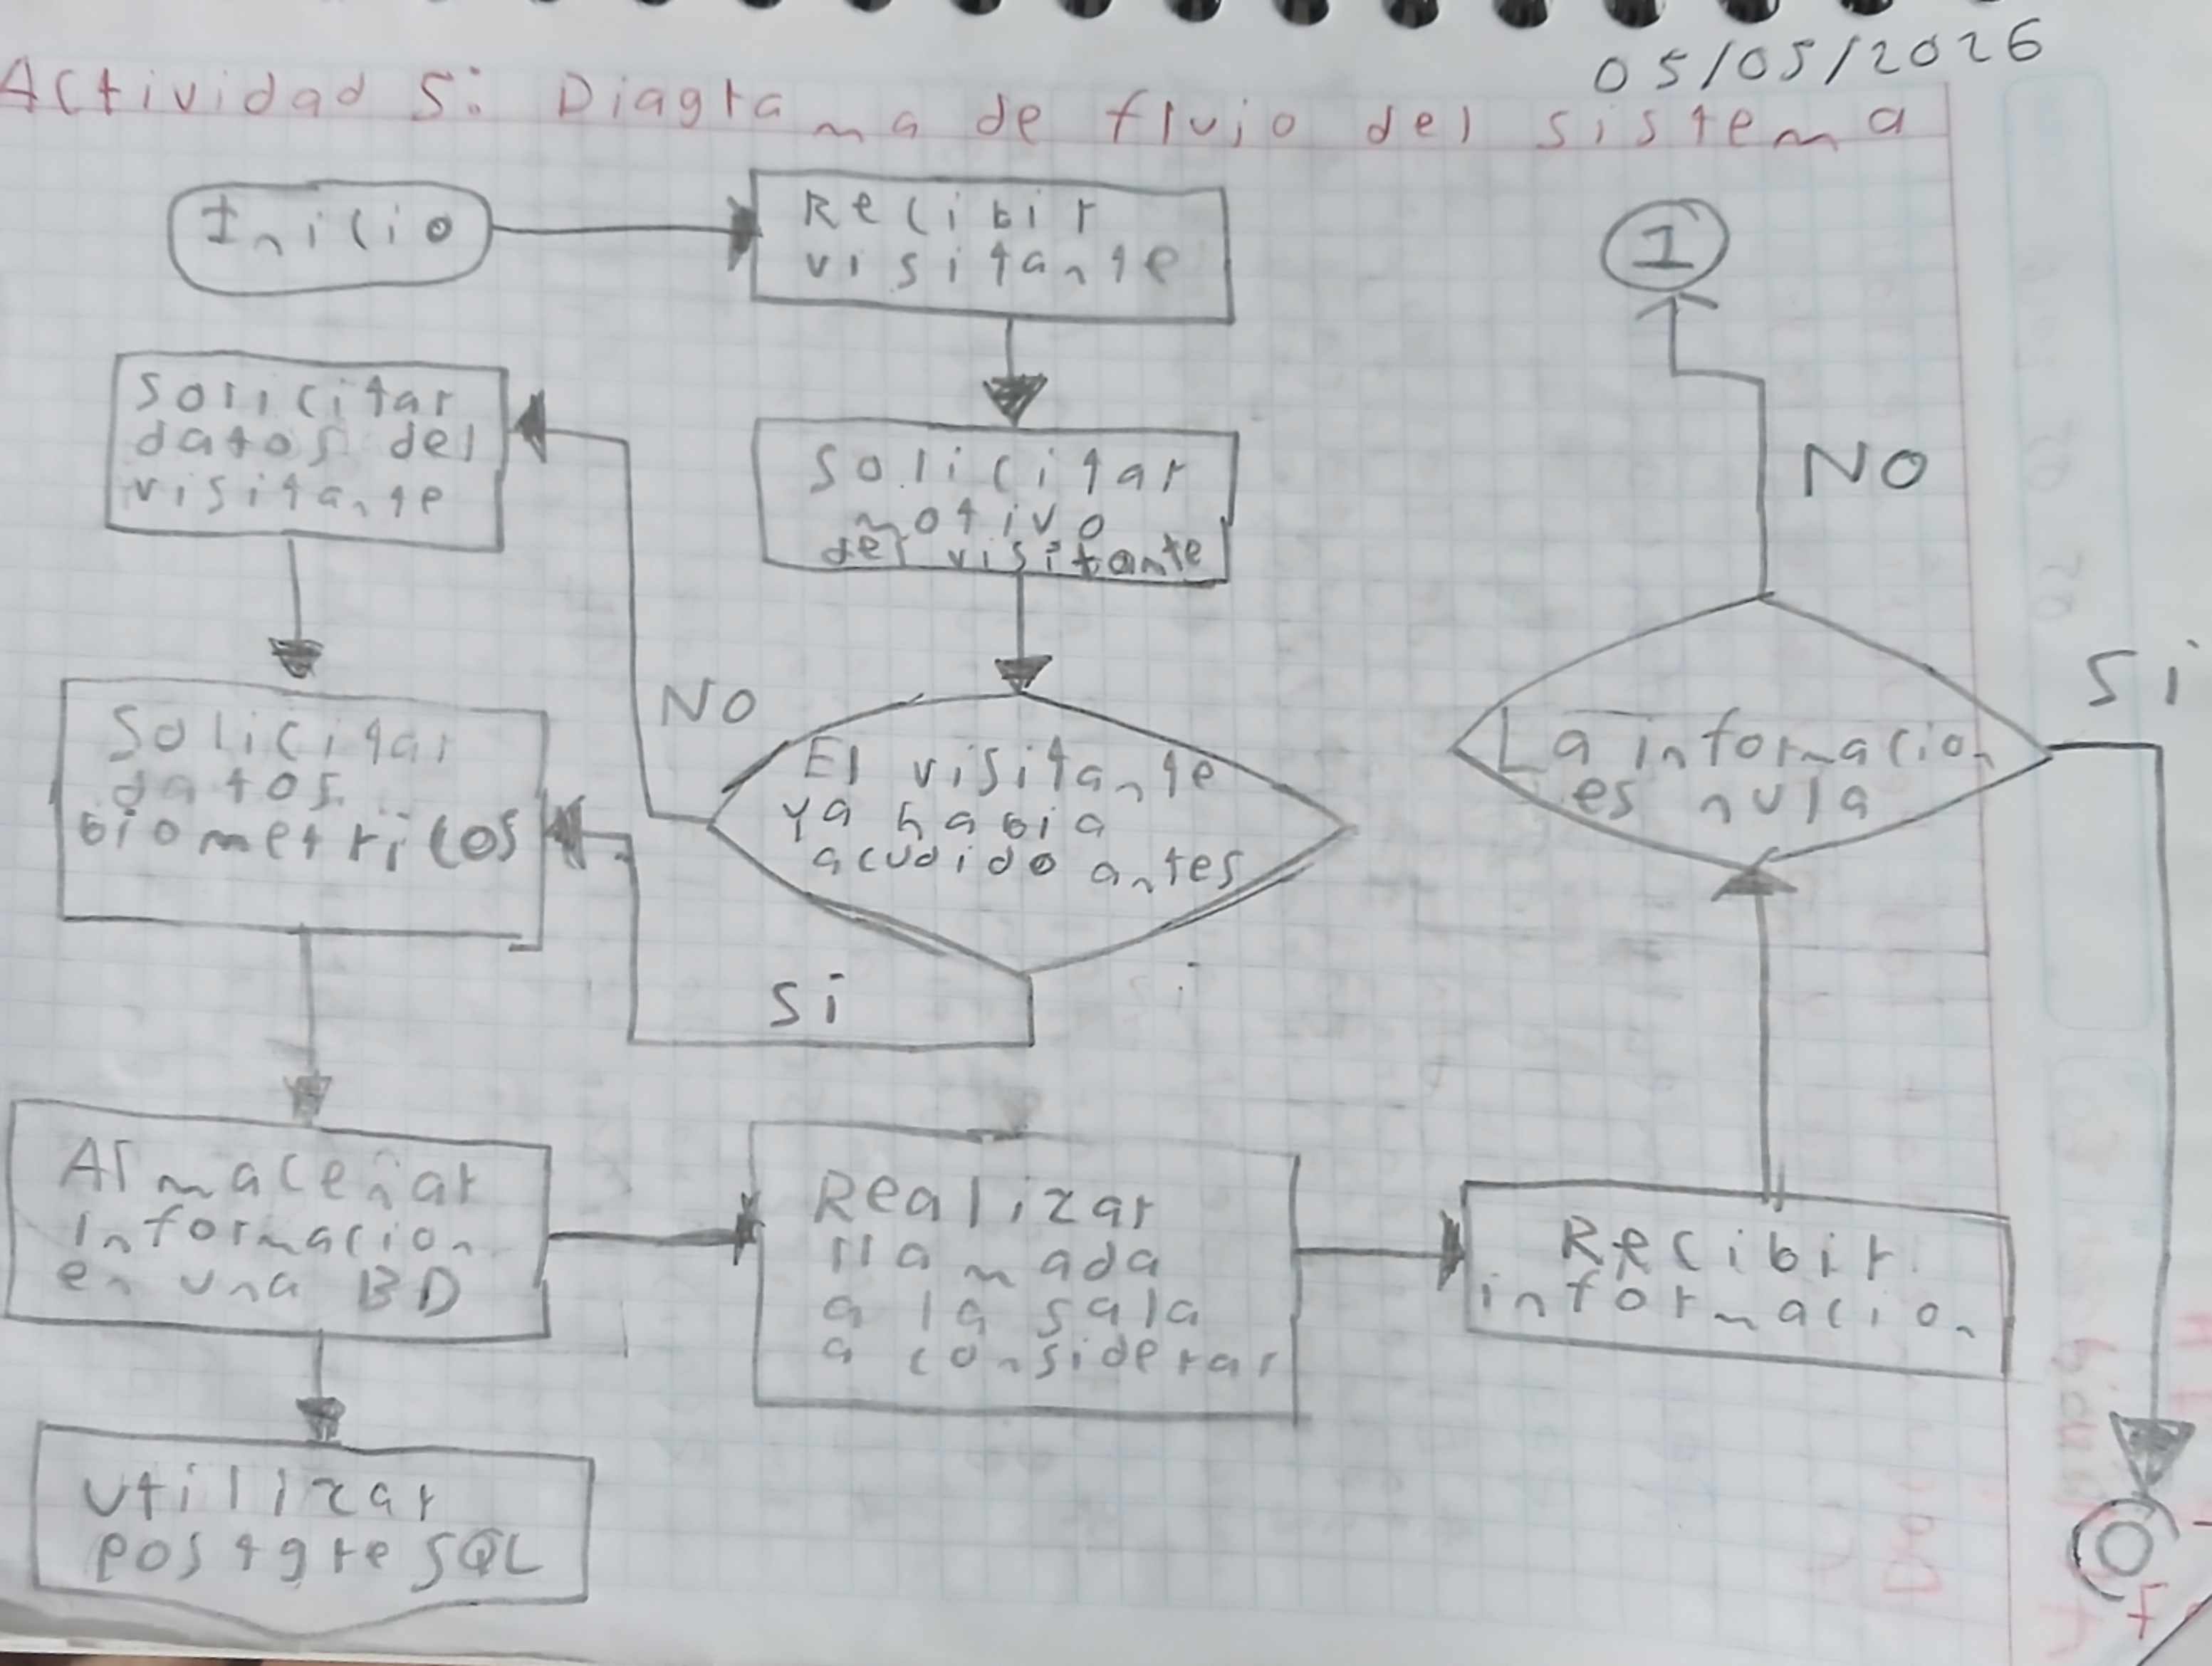
\includegraphics[width=0.9\linewidth]{figs/diagramaDeFlujo1.png}
    \caption{Diagrama de flujo del proyecto. Diagrama realizado por David Alejandro Ibarra Castañeda}
    \label{fig:DiagramaDeFlujoBasico}
\end{figure}

La figura \ref{fig:WireframesBasicos}, nos muestra los wireframes de baja fidelidad realizados. Ahí mismo vienen 3 interfaces clave para el proyecto, como la interfaz del registro de los visitantes, el panel de administración y la gestión de salas de la agencia.

\begin{figure}[H]
    \centering
    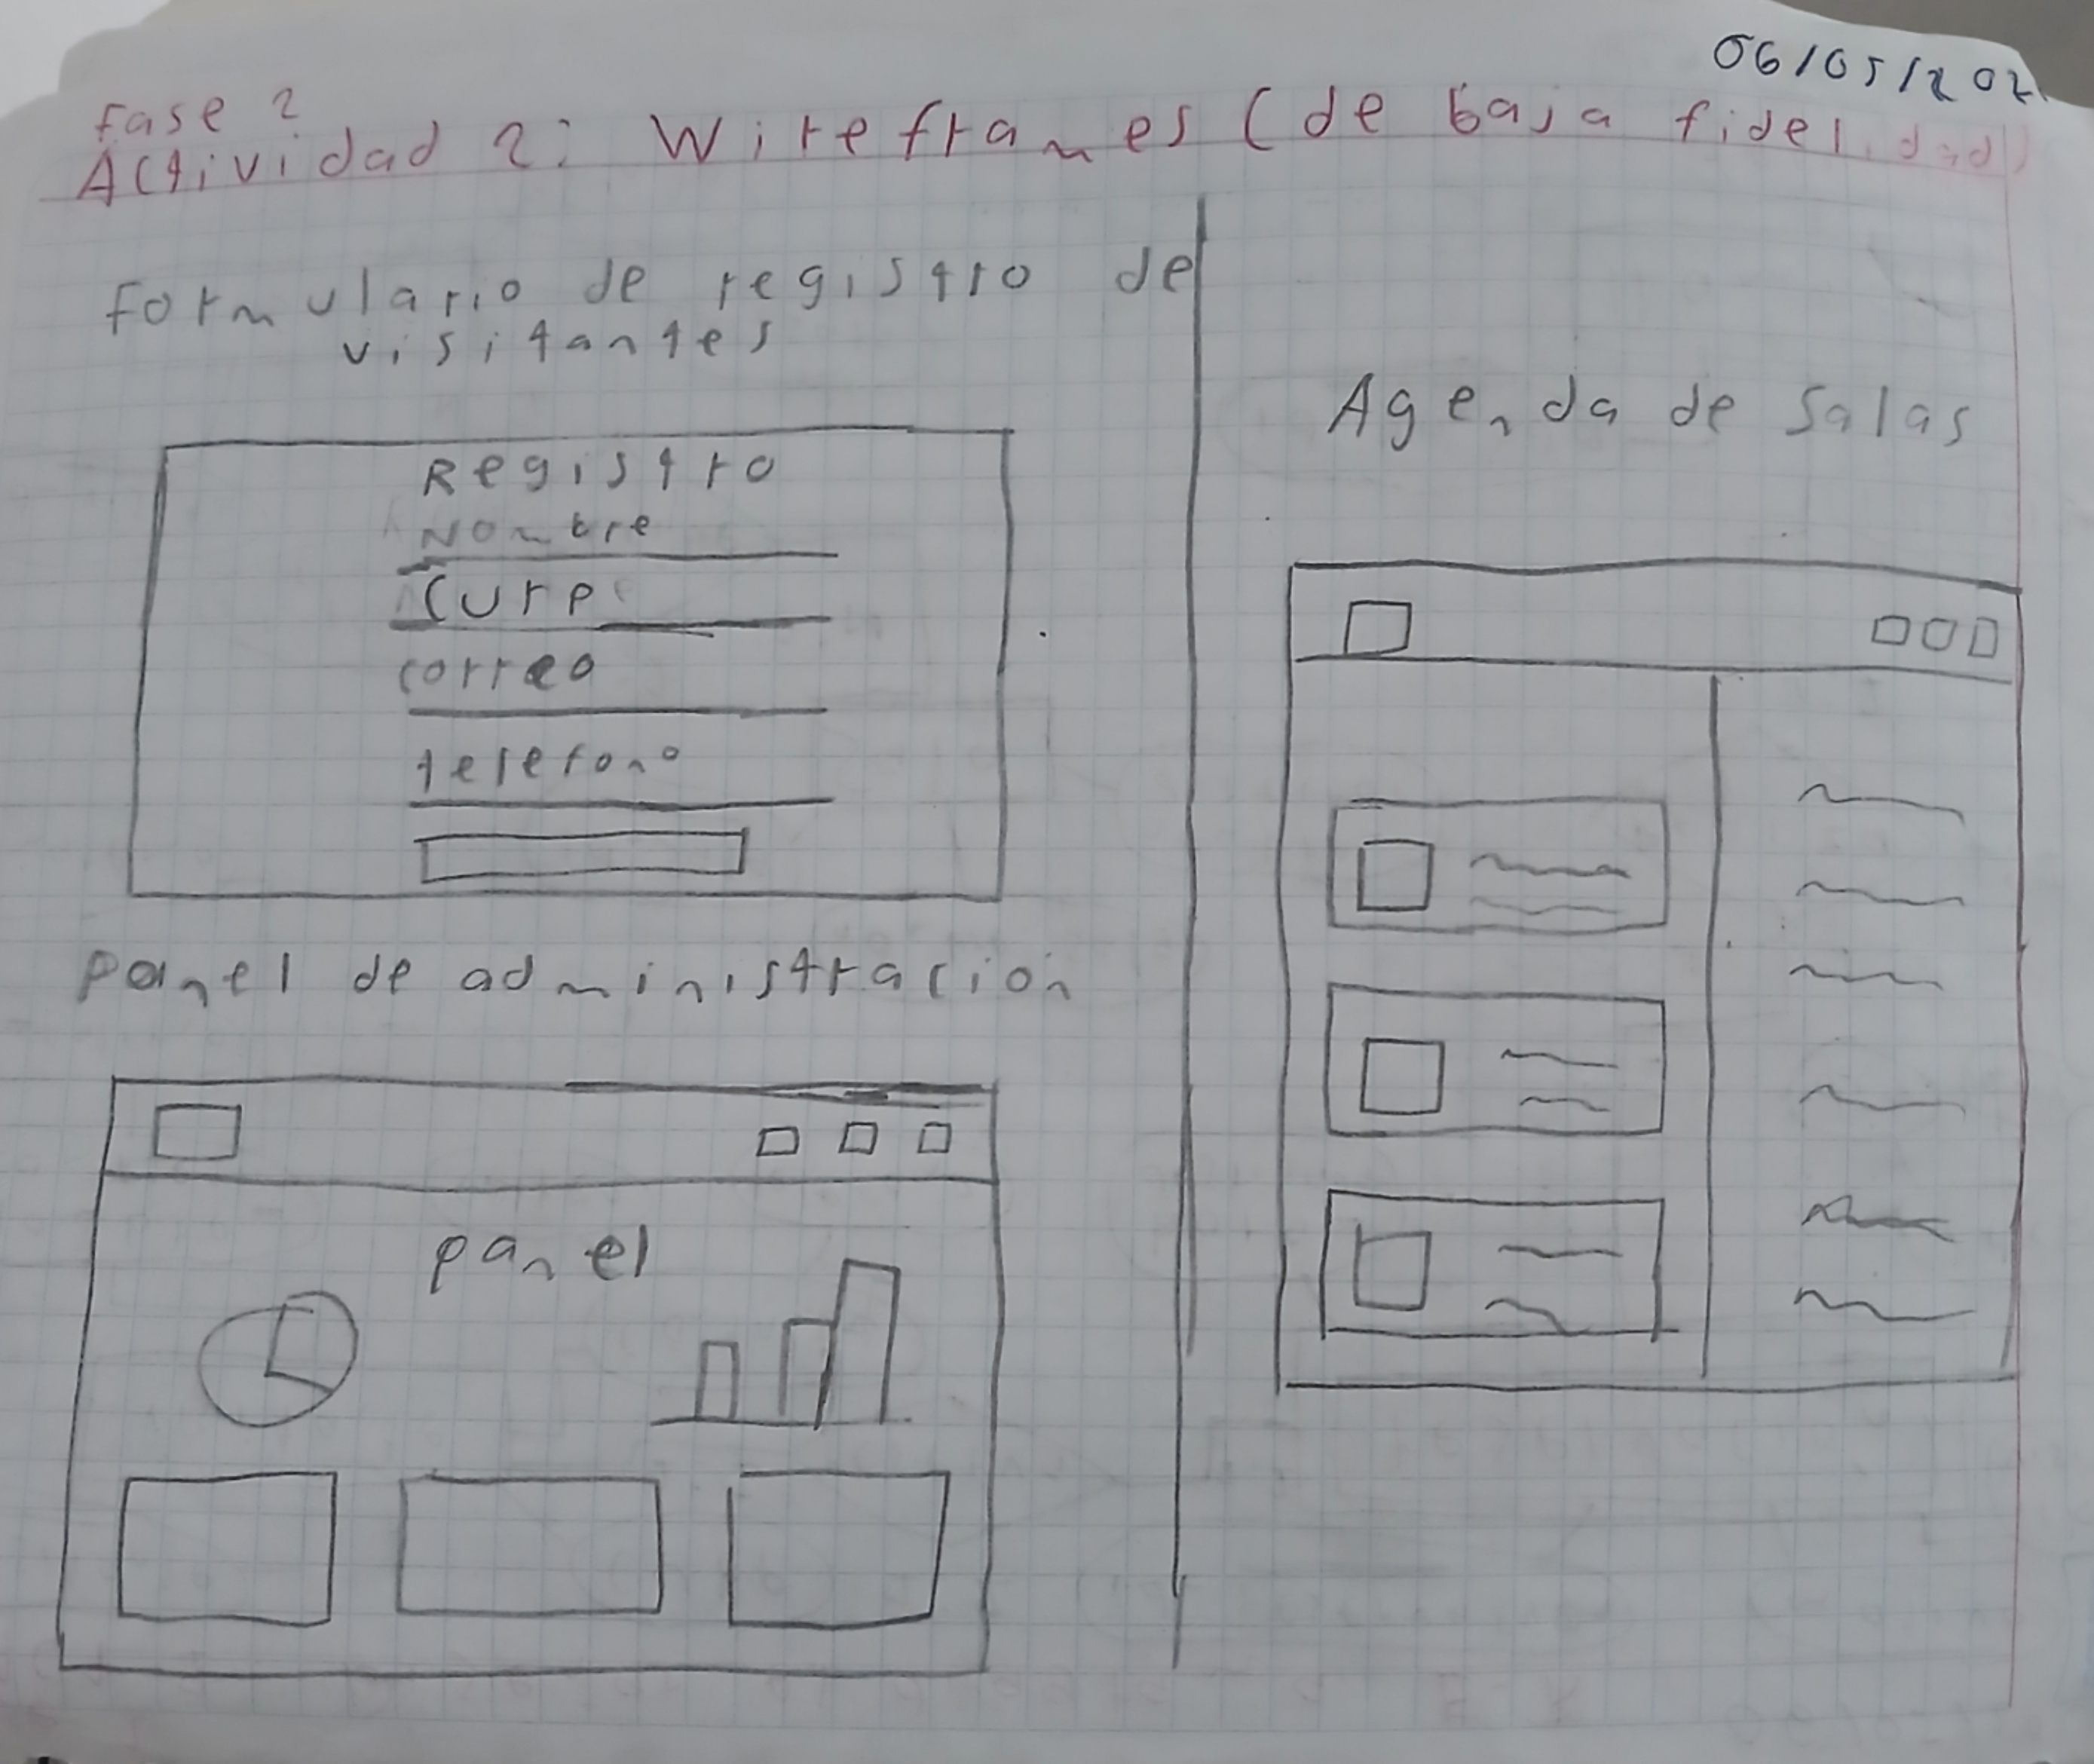
\includegraphics[width=0.9\linewidth]{figs/wireframes.png}
    \caption{Wireframes de baja fidelidad. Realizados por David Alejandro Ibarra Castañeda}
    \label{fig:WireframesBasicos}
\end{figure}

En la semana 4, me puse a diseñar algunos diagramas UML del proyecto.

Empezamos con el básico: El de Secuencia. La figura \ref{fig:DiagramaSecuencia}, muestra el ciclo de vida del sistema, los involucrados en el y como estos van interactuando entre si. Esta mas enfocado al registro de los visitantes.

\begin{figure}[H]
    \centering
    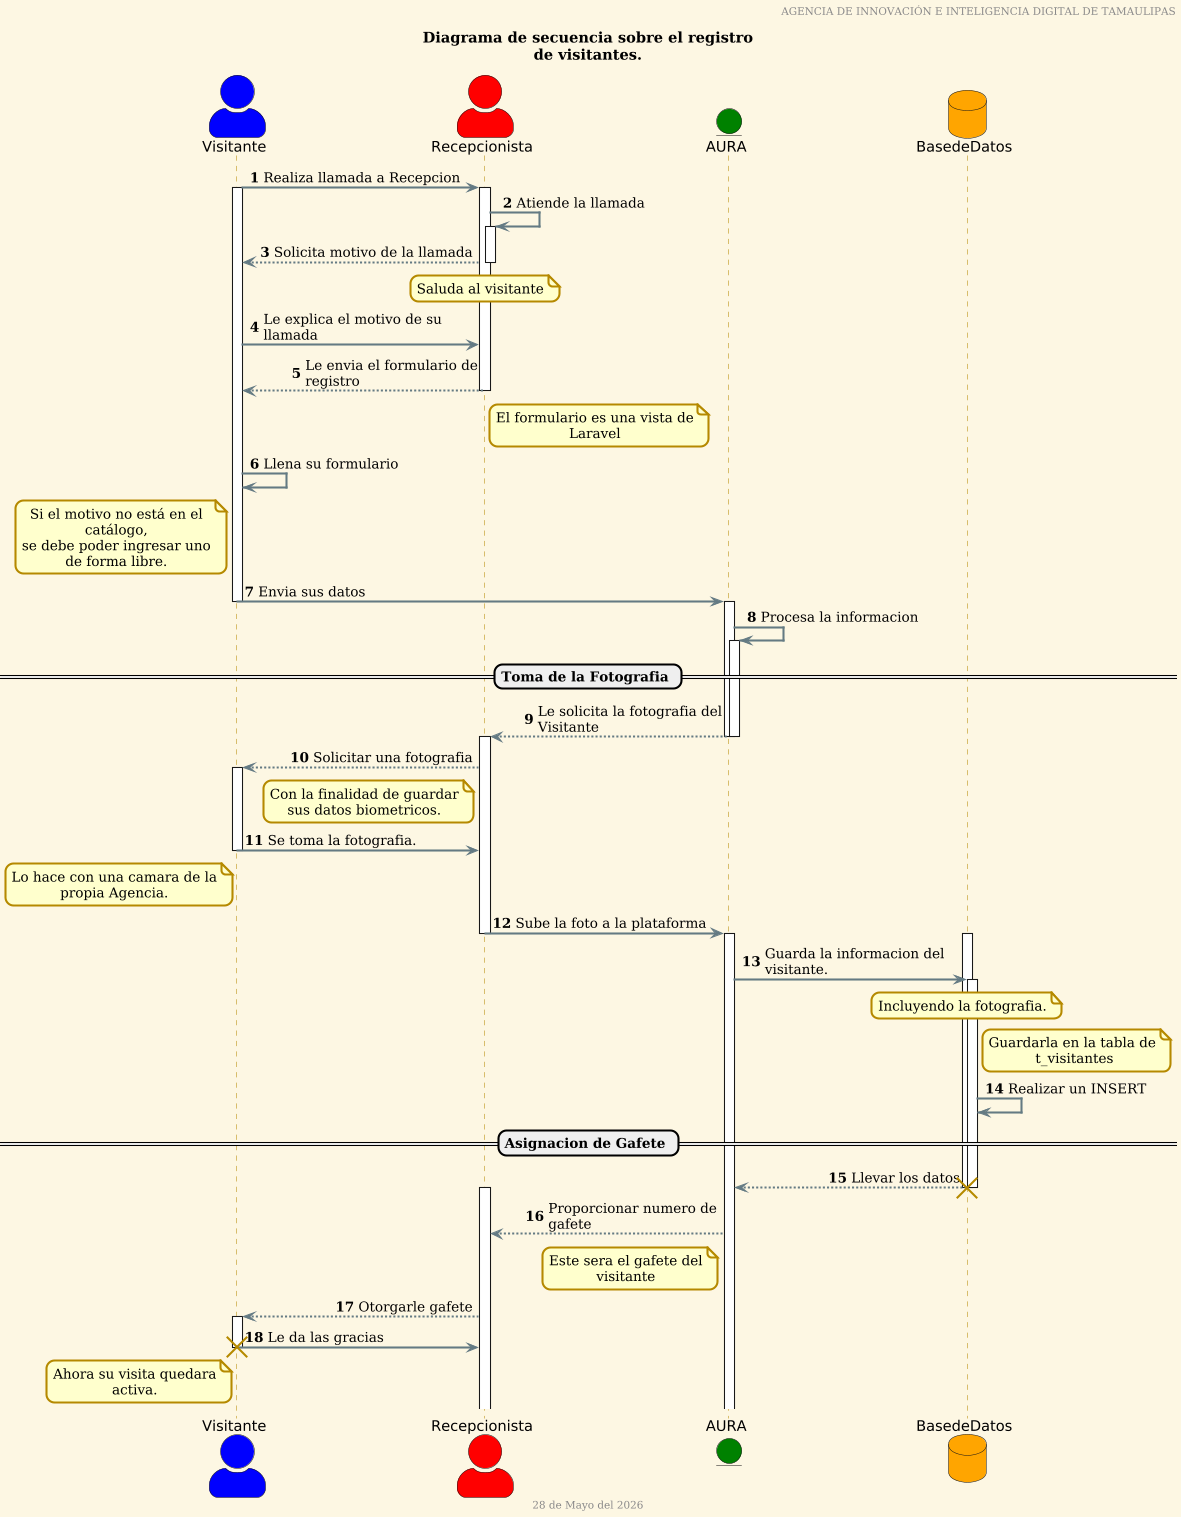
\includegraphics[width=0.9\linewidth]{figs/DiagramaDeSecuencia.png}
    \caption{Diagrama de Secuencia del proyecto. Diseñado por David Alejandro Ibarra Castañeda}
    \label{fig:DiagramaSecuencia}
\end{figure}

En la figura \ref{fig:DiagramaDeFlujoFinal}, podemos visualizar el verdadero diagrama de flujo del proyecto. Al igual que el anterior diagrama de flujo, este esta enfocado en el registro de visitantes, solo que esta vez, es la versión final del diseño.

\begin{figure}[H]
    \centering
    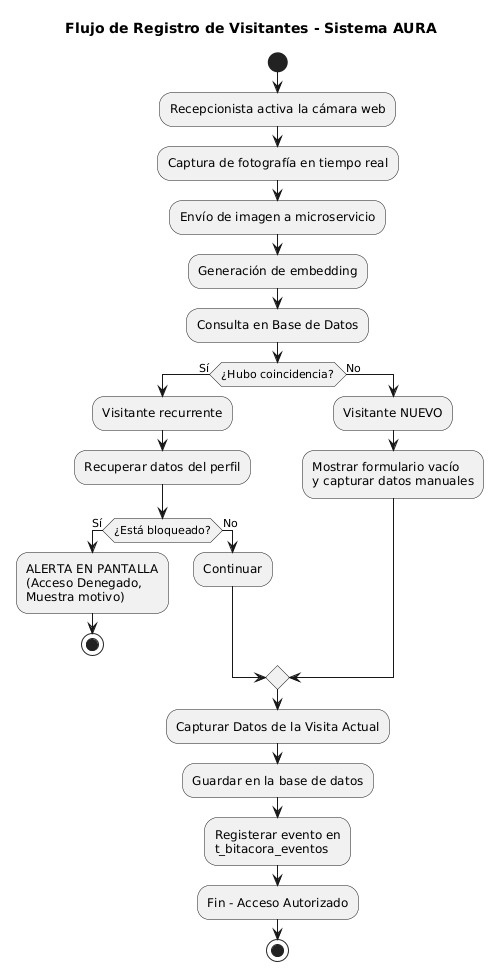
\includegraphics[width=0.4\linewidth]{figs/DiagramaDeFlujo.jpg}
    \caption{Diagrama de flujo final. Diseñado por David Alejandro Ibarra Castañeda}
    \label{fig:DiagramaDeFlujoFinal}
\end{figure}

\clearpage

Ahora pasemos a ver algunos diagramas tecnicos... empezando con el diagrama \textit{ER} (Entidad-Relación). La figura \ref{fig:DiagramaER}, muestra a detalle este diagrama. La empresa tiene nomenclaturas claras a la hora de renombrar las tablas... por ejemplo, los catálogos se renombran con una C, junto con un guion bajo y enseguida el nombre. Lo mismo con las tablas, solo reemplazamos la c por una t.

\begin{figure}[H]
    \centering
    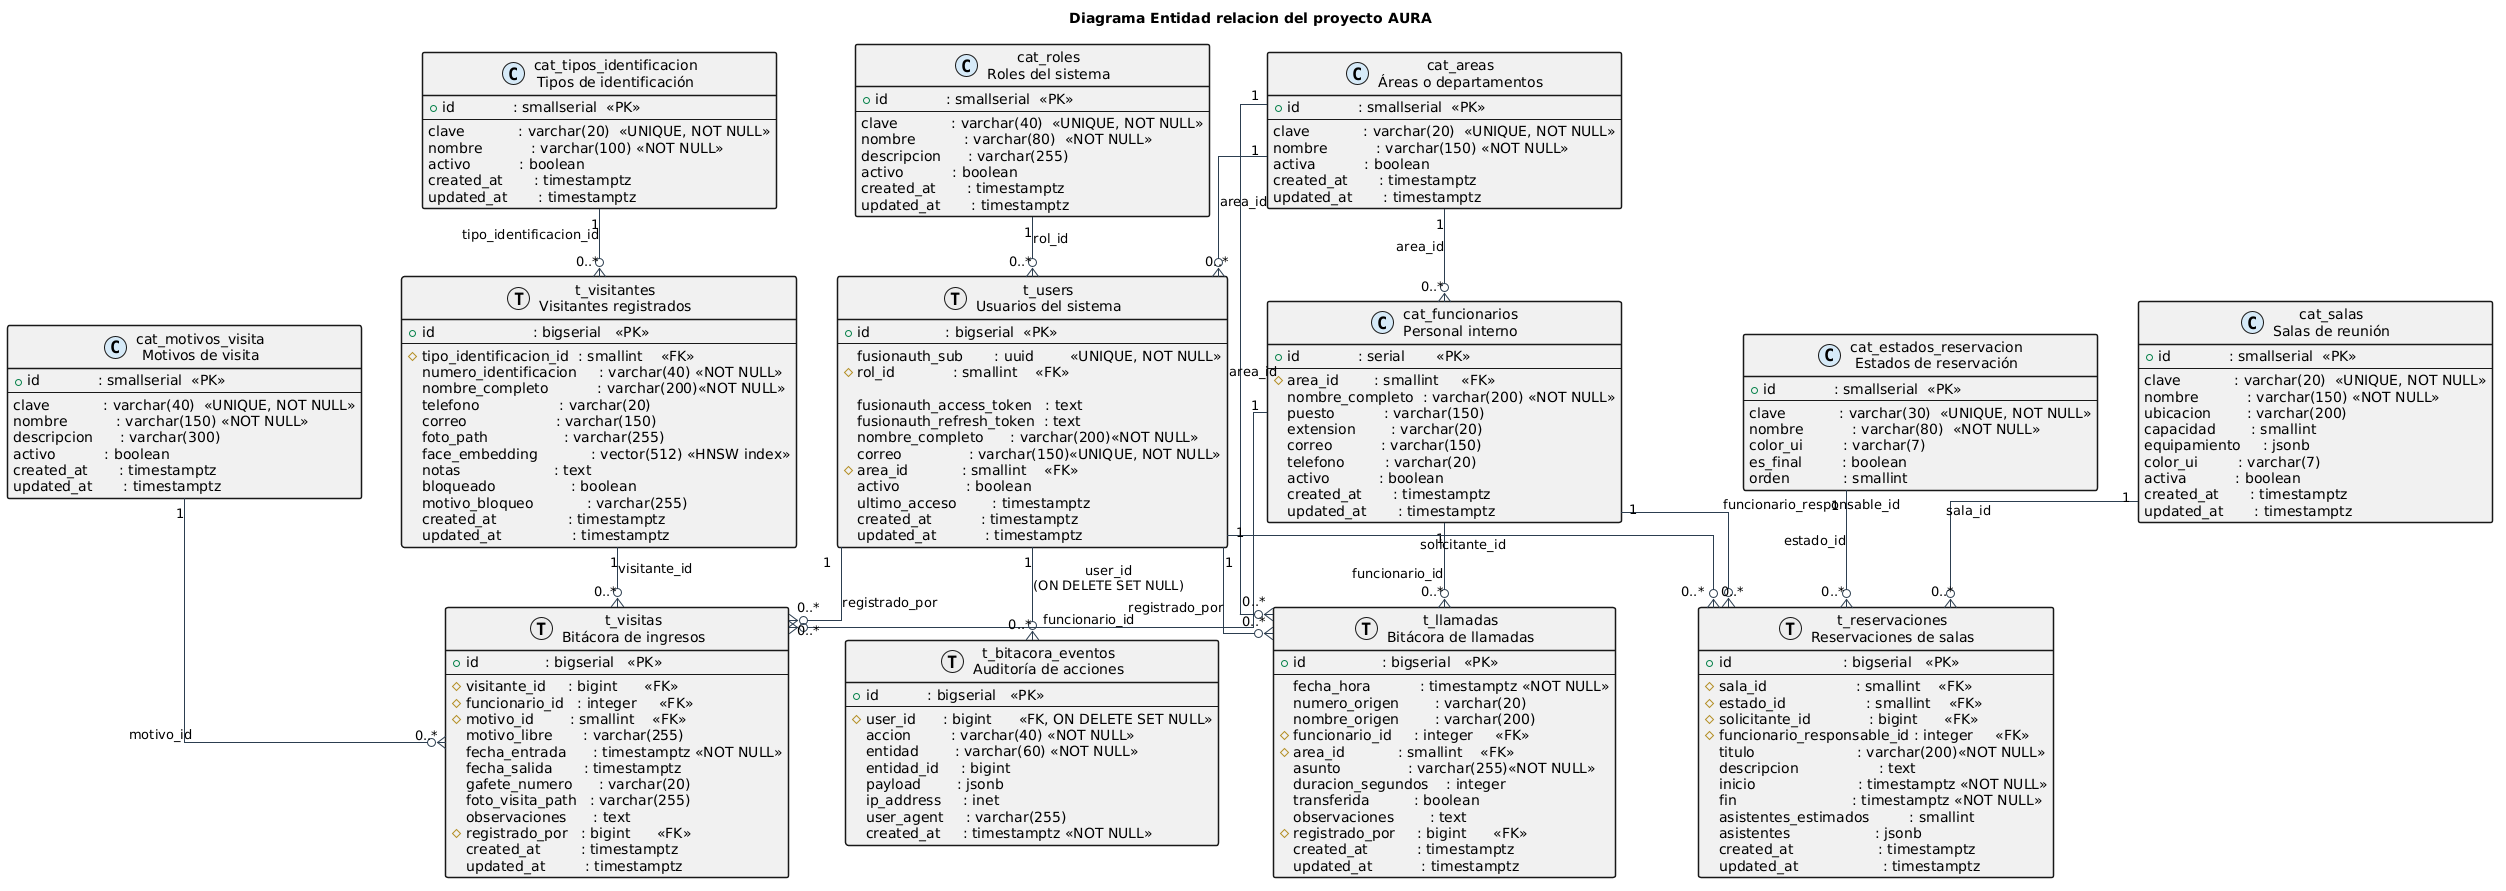
\includegraphics[width=0.9\linewidth]{figs/DiagramaER.png}
    \caption{Diagrama ER del proyecto. Diseñado por David Alejandro Ibarra Castañeda}
    \label{fig:DiagramaER}
\end{figure}

En la figura \ref{fig:DiagramaDeComponentes}, podemos ver los componentes que va estar utilizando el sistema y como estos van a estar interactuando entre si.

\begin{figure}[H]
    \centering
    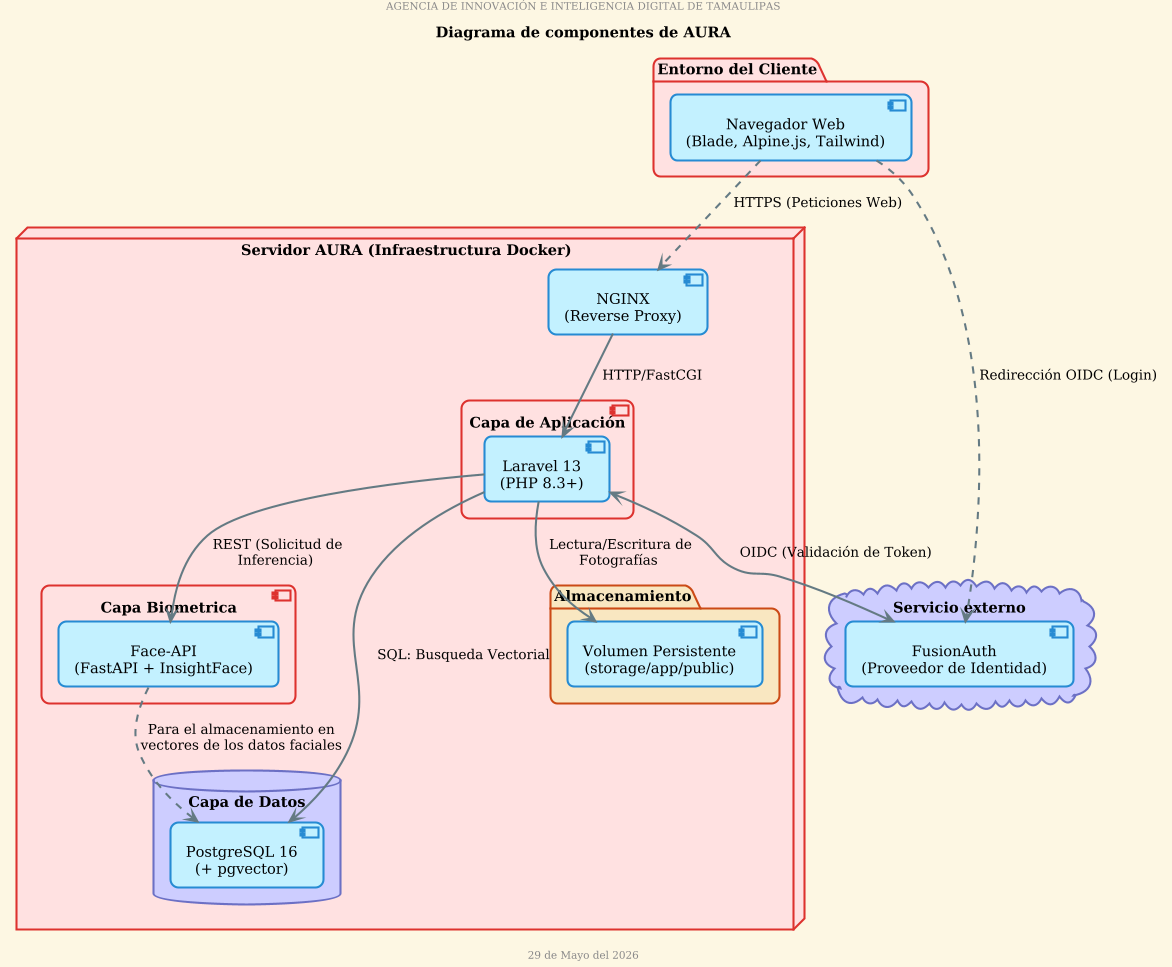
\includegraphics[width=0.9\linewidth]{figs/DiagramaDeComponentes.png}
    \caption{Diagrama de componentes en UML. Diseñado por David Alejandro Ibarra Castañeda}
    \label{fig:DiagramaDeComponentes}
\end{figure}


En la semana 5, comencé a desarrollar ahora si que los wireframes de alta fidelidad para la plataforma. Los wireframes fueron realizados en Figma. En la figura \ref{fig:Login}, veremos la primera interfaz realizada: El login de la plataforma.

\begin{figure}[H]
    \centering
    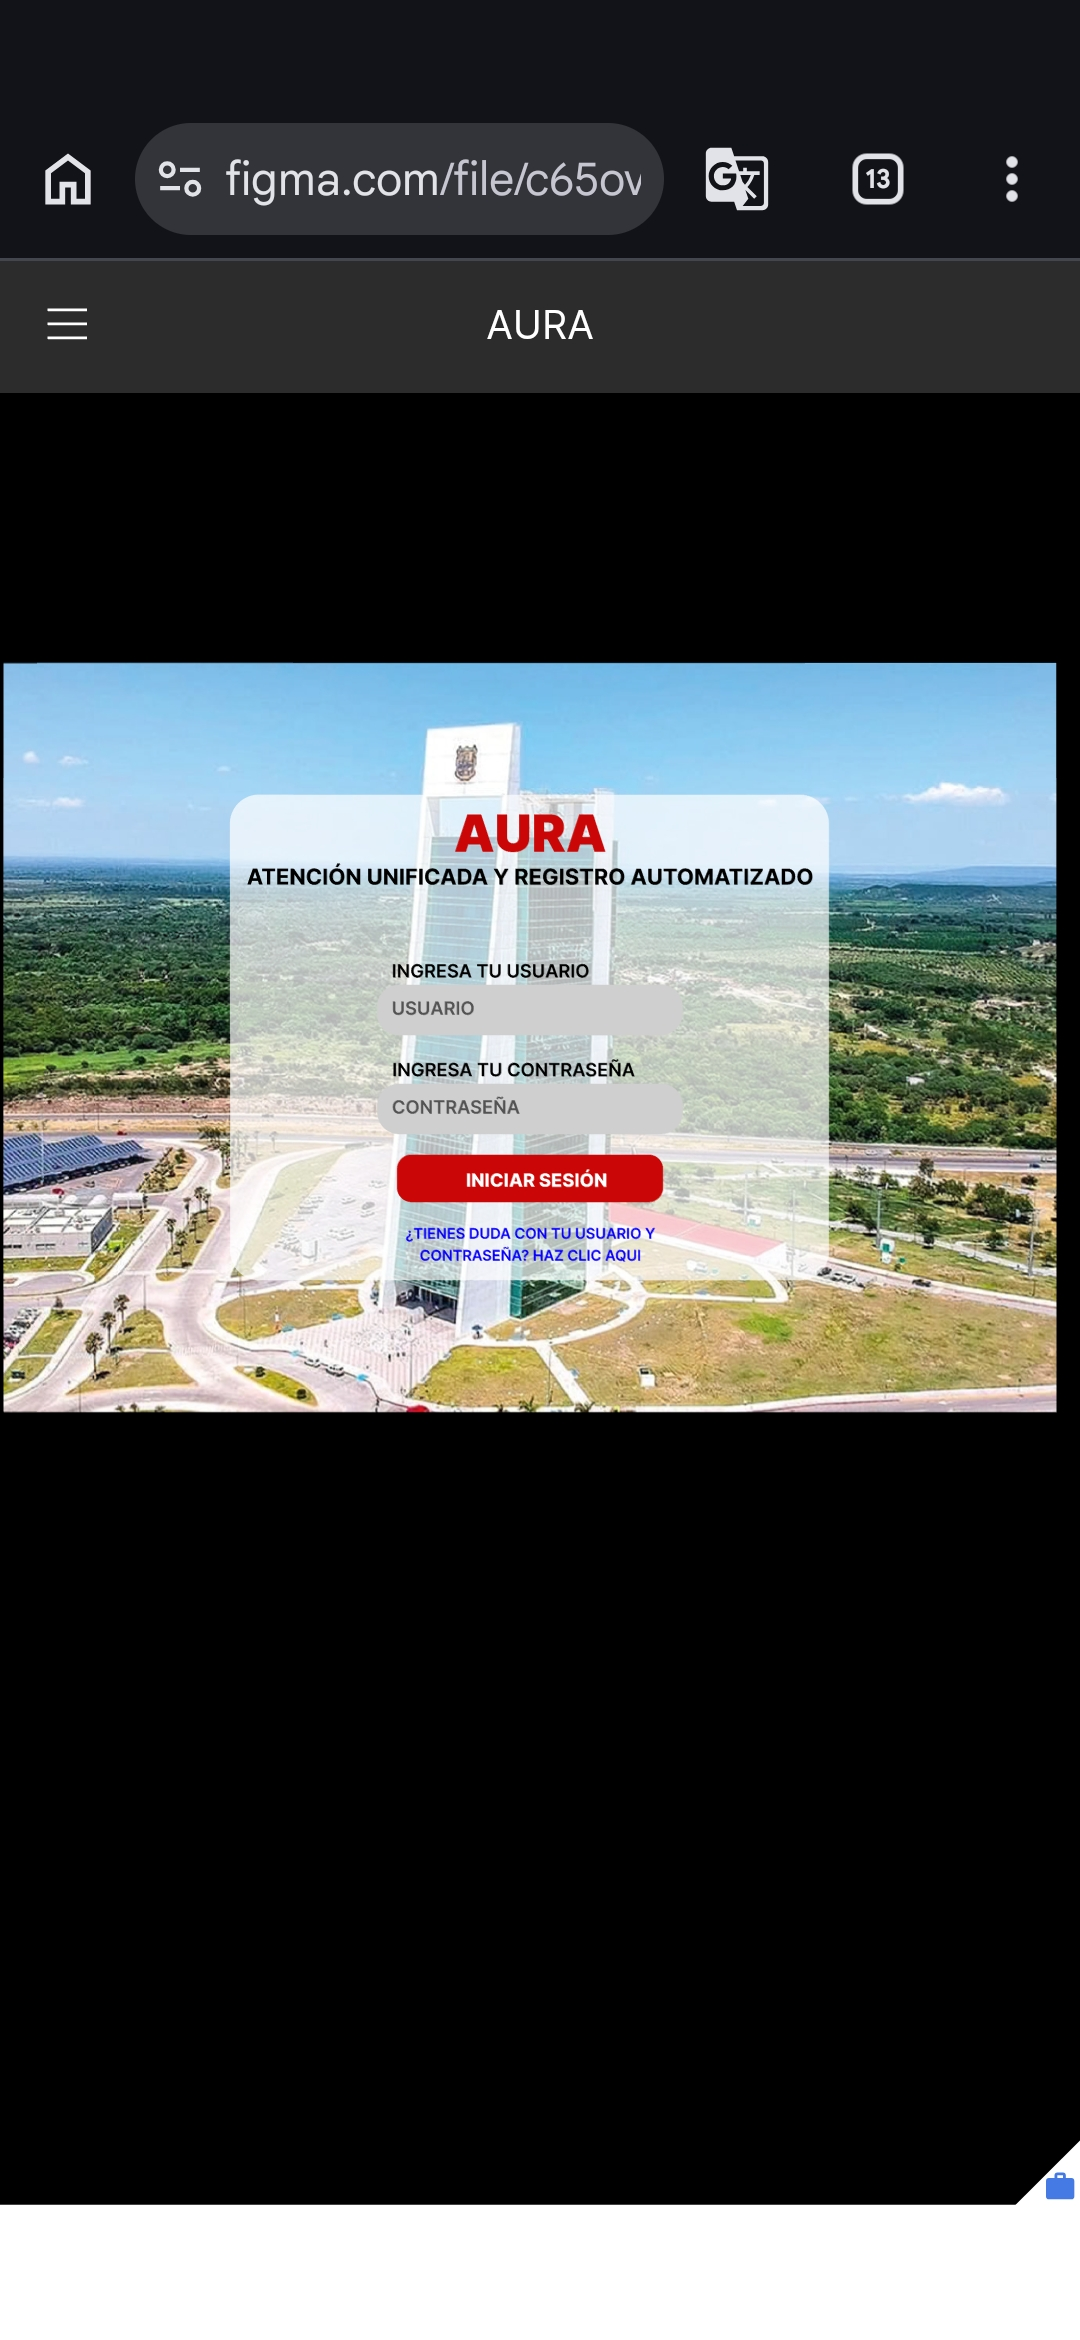
\includegraphics[width=0.4\linewidth]{figs/Login.jpg}
    \caption{Login de la plataforma. Diseñado en Figma}
    \label{fig:Login}
\end{figure}

Por supuesto, la figura \ref{fig:Dashboard}, muestra como la plataforma cuenta con su propio dashboard... para la visualización de visitas recurrentes, cantidad de visitantes en la unidad económica y sobre las acciones que podrían realizar los usuarios en la plataforma.

\begin{figure}[H]
    \centering
    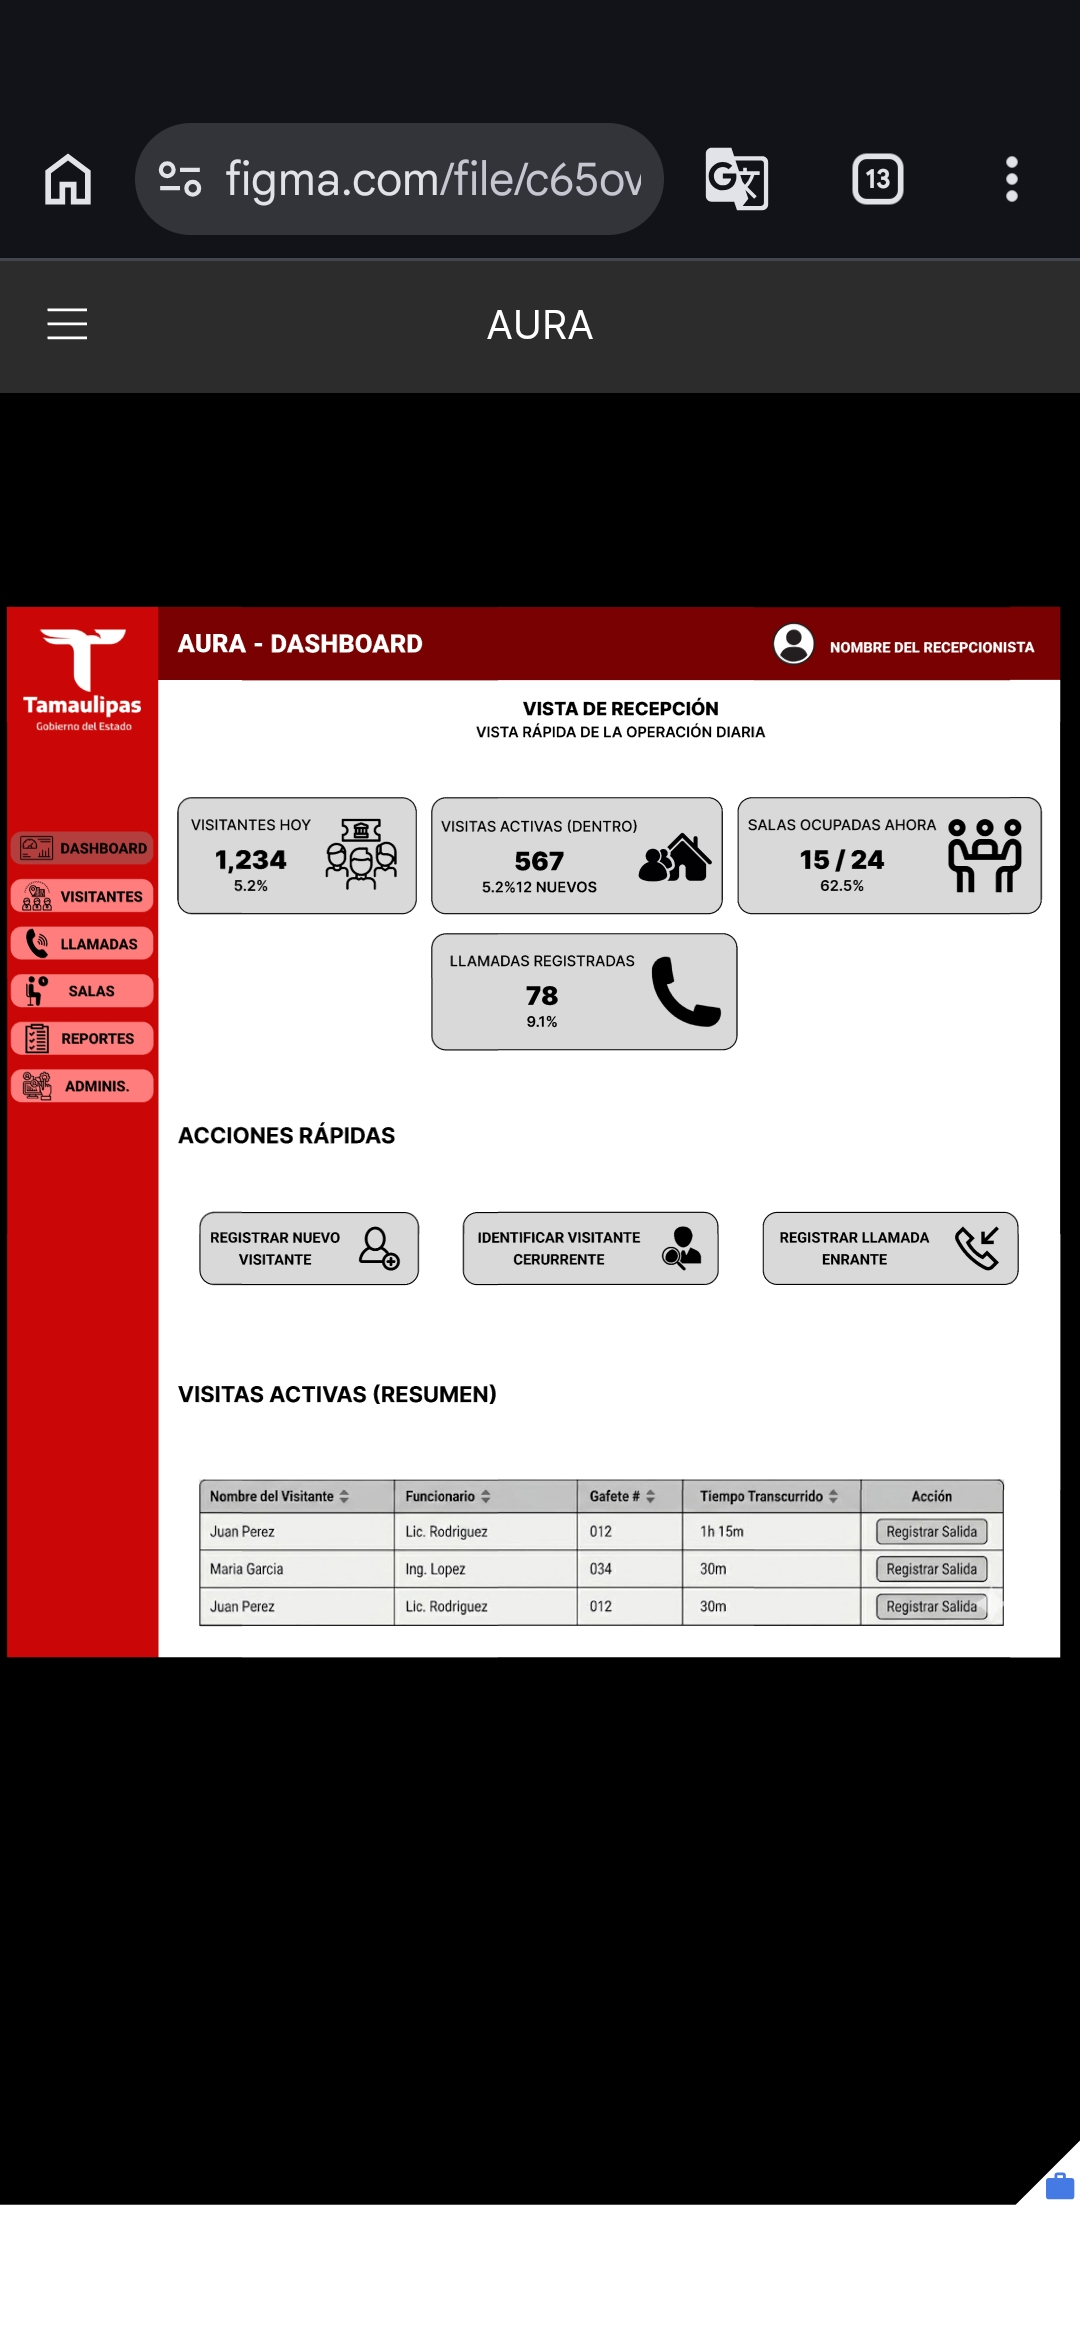
\includegraphics[width=0.4\linewidth]{figs/Dashboard.jpg}
    \caption{Dashboard de la plataforma. Diseñado en Figma}
    \label{fig:Dashboard}
\end{figure}


A continuación, la figura \ref{fig:Registro-visitantes} muestra el modulo de visitantes, en donde los usuarios podrán registrar a las visitas que van llegando a la agencia. También la interfaz cuenta con un apartado para la toma de la fotografía del visitante, para así poder agilizar el proceso de búsqueda del visitante con tan solo buscar su rostro mediante embenddings en vez de ir escribiendo los datos del visitante manualmente. Aquí le asignamos el funcionario a visitar, motivo de visita, motivo libre y su gafete.

\begin{figure}[H]
    \centering
    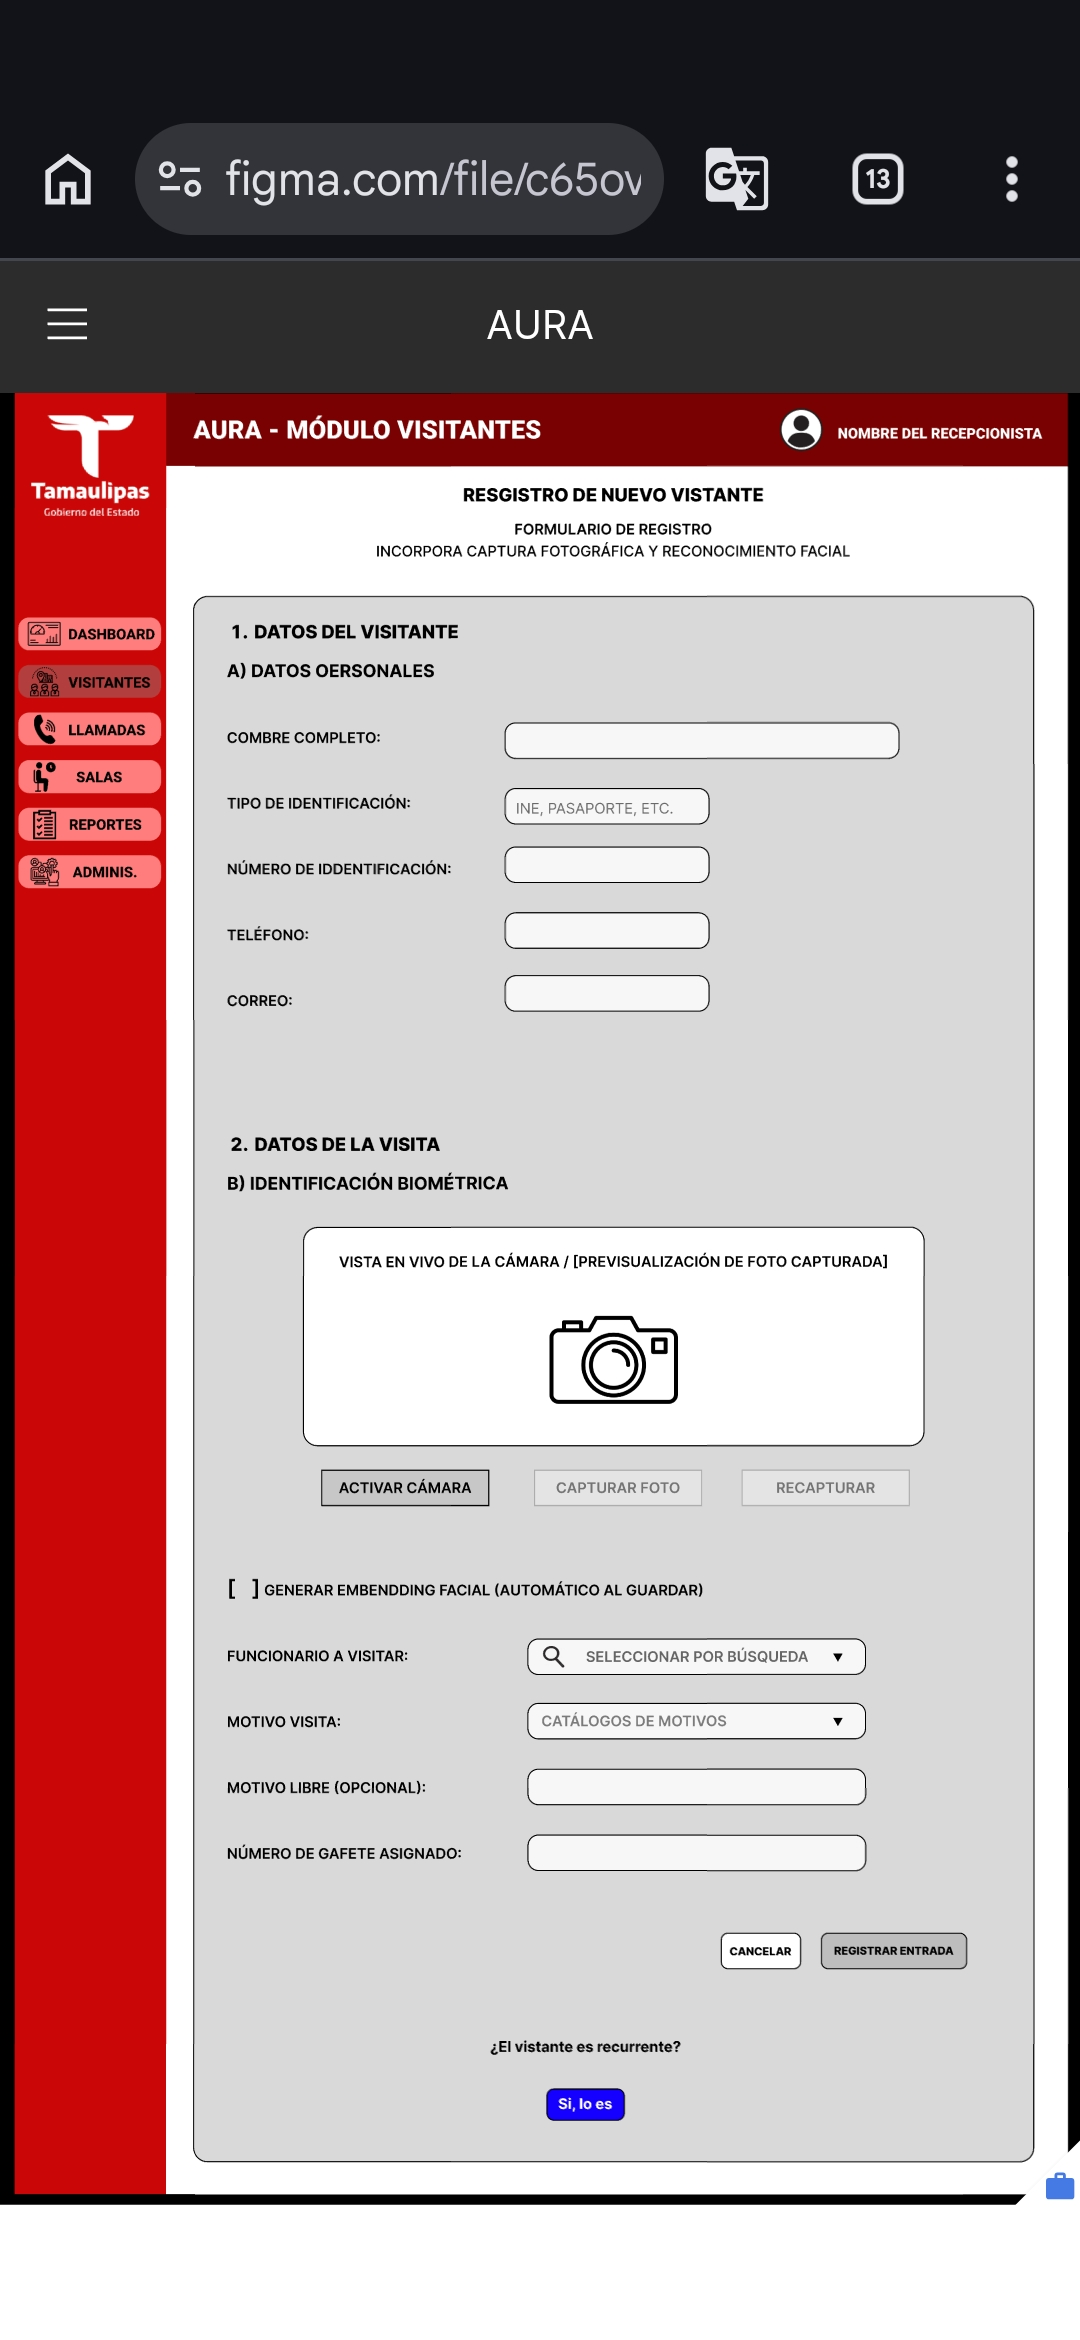
\includegraphics[width=0.6\linewidth]{figs/Registro-visitantes.jpg}
    \caption{Modulo de registro de visitantes. Diseñado en Figma}
    \label{fig:Registro-visitantes}
\end{figure}

Si nuestro visitante suele acudir mucho a la agencia del piso 2, recepción le pedirá al visitante la fotografía, para que de esta forma, los usuarios de la plataforma puedan encontrar a la persona mas rápido. La figura \ref{fig:Reconocimientofacial}, nos muestra el wireframe correspondiente.

\begin{figure}[H]
    \centering
    
\includegraphics[width=0.4\linewidth]{figs/Reconocimientofacial.jpg}
    \caption{Sistema de captura facial para la recepción de la Agencia. Diseñado en Figma}
    \label{fig:Reconocimientofacial}
\end{figure}

Recepción necesita registrar las llamadas que van recibiendo por parte de los visitantes, es por eso que la figura \ref{fig:Gestion-llamadas}, nos muestra una interfaz para la gestión de las llamadas entrantes.

\begin{figure}[H]
    \centering
    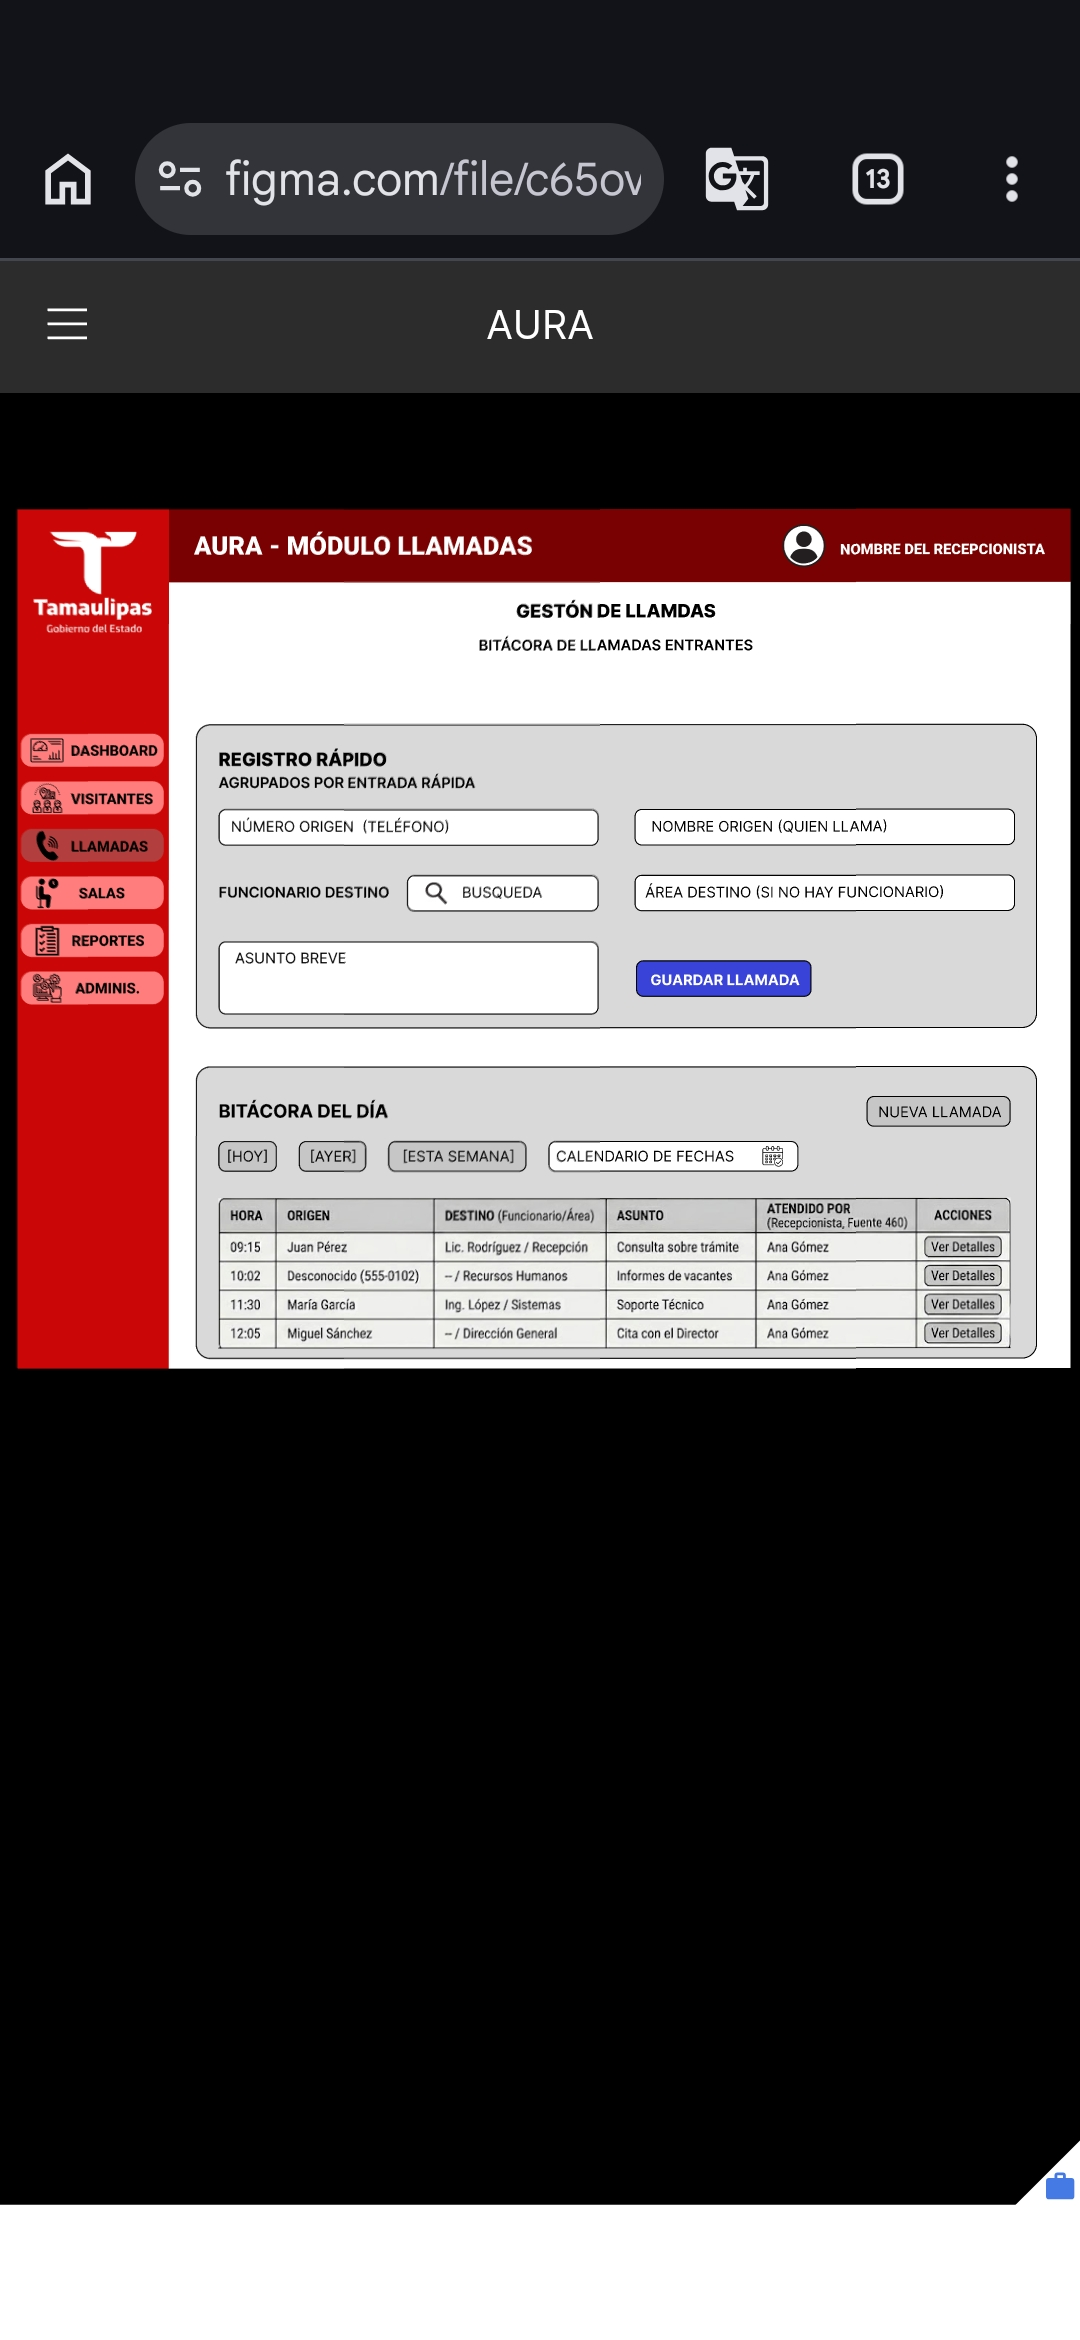
\includegraphics[width=0.4\linewidth]{figs/Gestion-llamadas.jpg}
    \caption{UI pars la gestion de las llamadas de la plataforma. Diseñado en Figma}
    \label{fig:Gestion-llamadas}
\end{figure}

La plataforma cuenta con un modulo de gestión de salas... fundamental para cuando un visitante quiera reservar una sala. En la figura \ref{fig:Gestion-salas}, se detalla el wireframe de este modulo.

\begin{figure}[H]
    \centering
    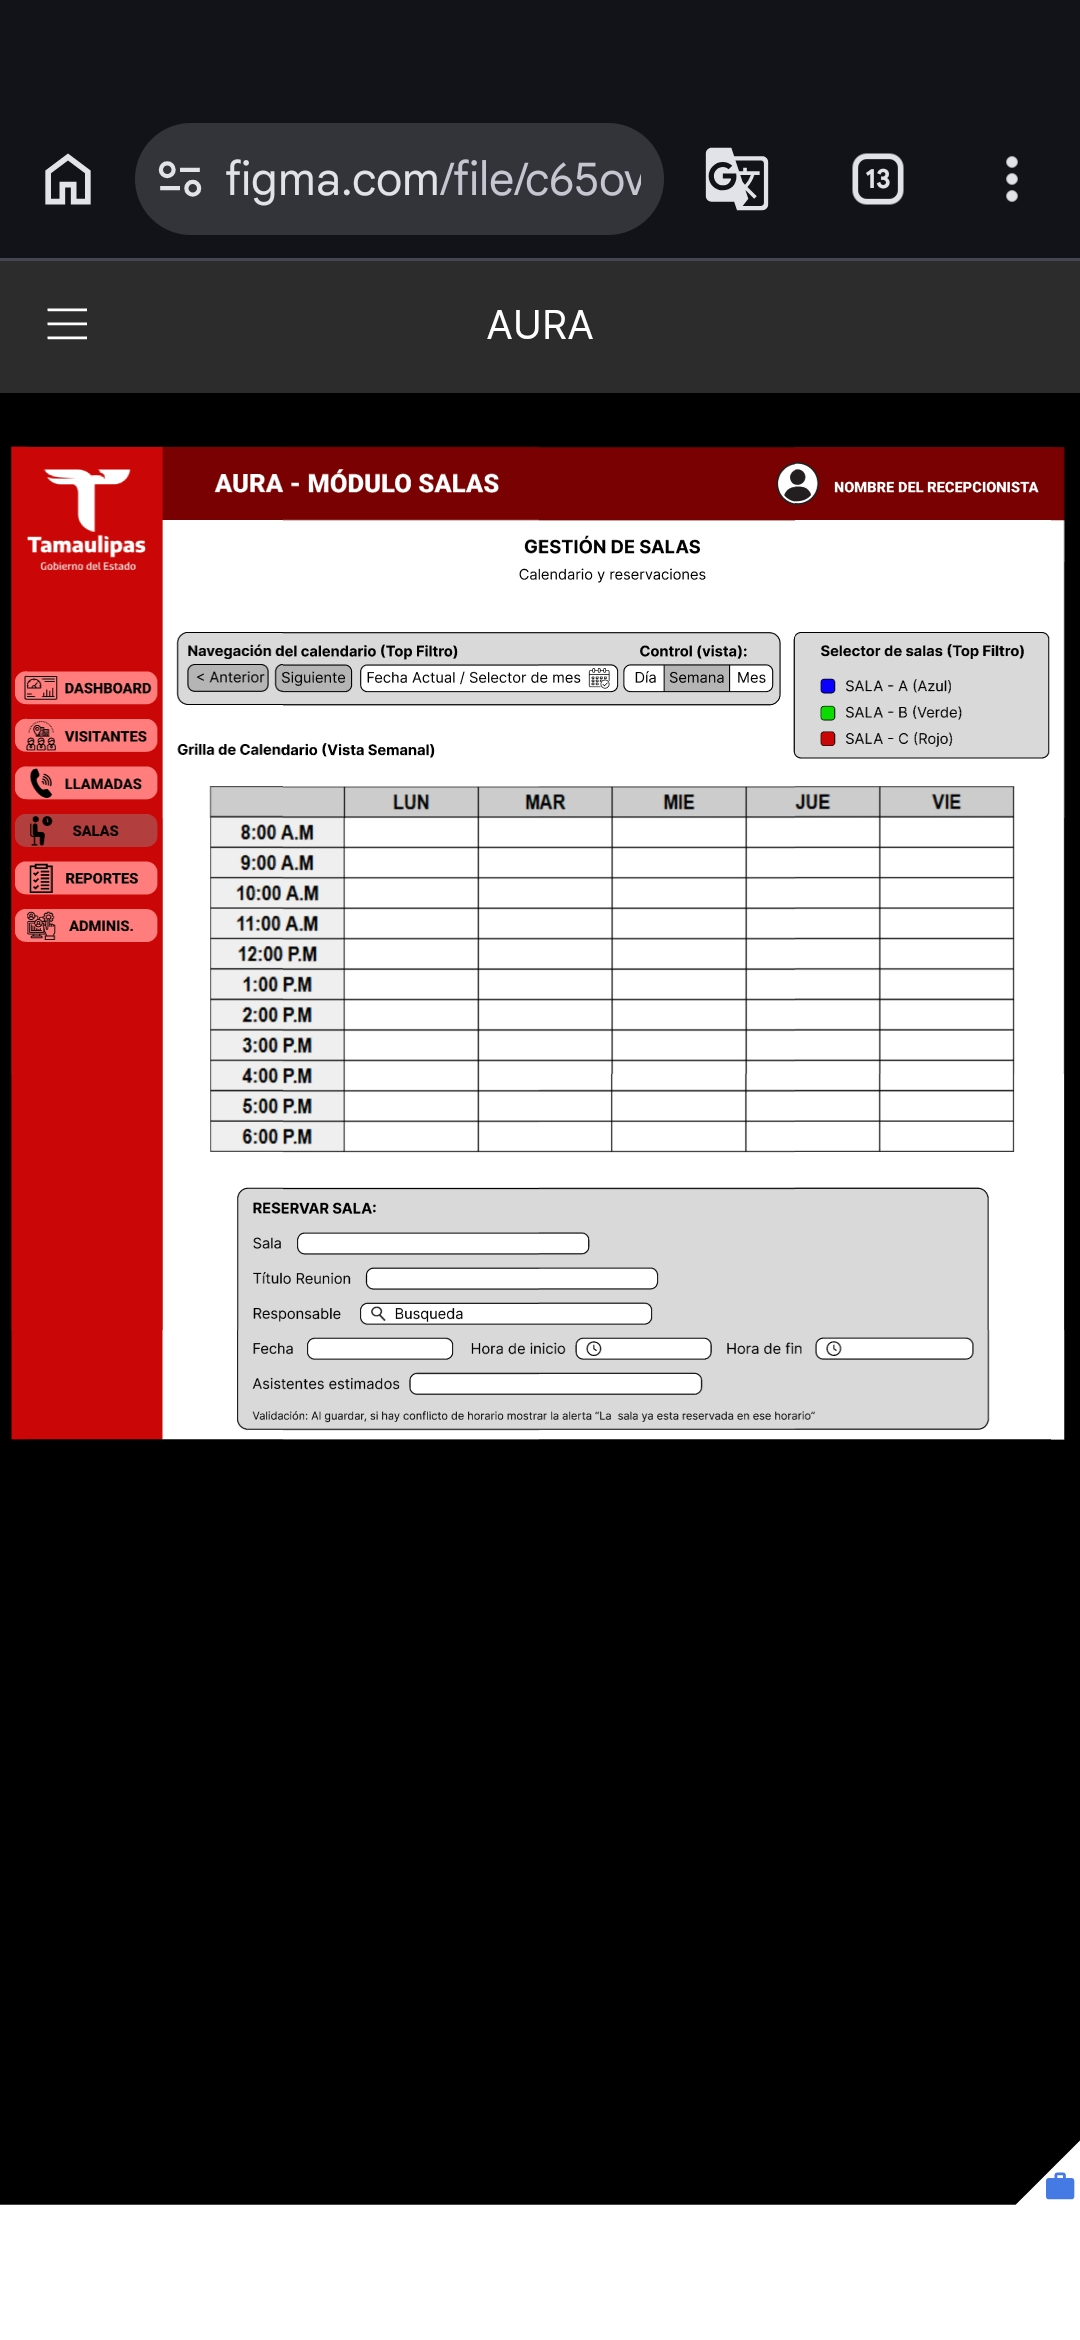
\includegraphics[width=0.4\linewidth]{figs/Gestion-salas.jpg}
    \caption{Gestión de las salas dentro de la plataforma. Diseñado en Figma}
    \label{fig:Gestion-salas}
\end{figure}

Por ultimo, la agencia debe ser capaz de realizar reportes sobre todos los datos que van almacenando, al igual que ver las salas que están ocupadas, realizar bitácoras de eventos y filtrar las reservaciones de los visitantes. En la figura \ref{fig:Reportes}, se encuentra la UI de la generación de los reportes.

\begin{figure}[H]
    \centering
    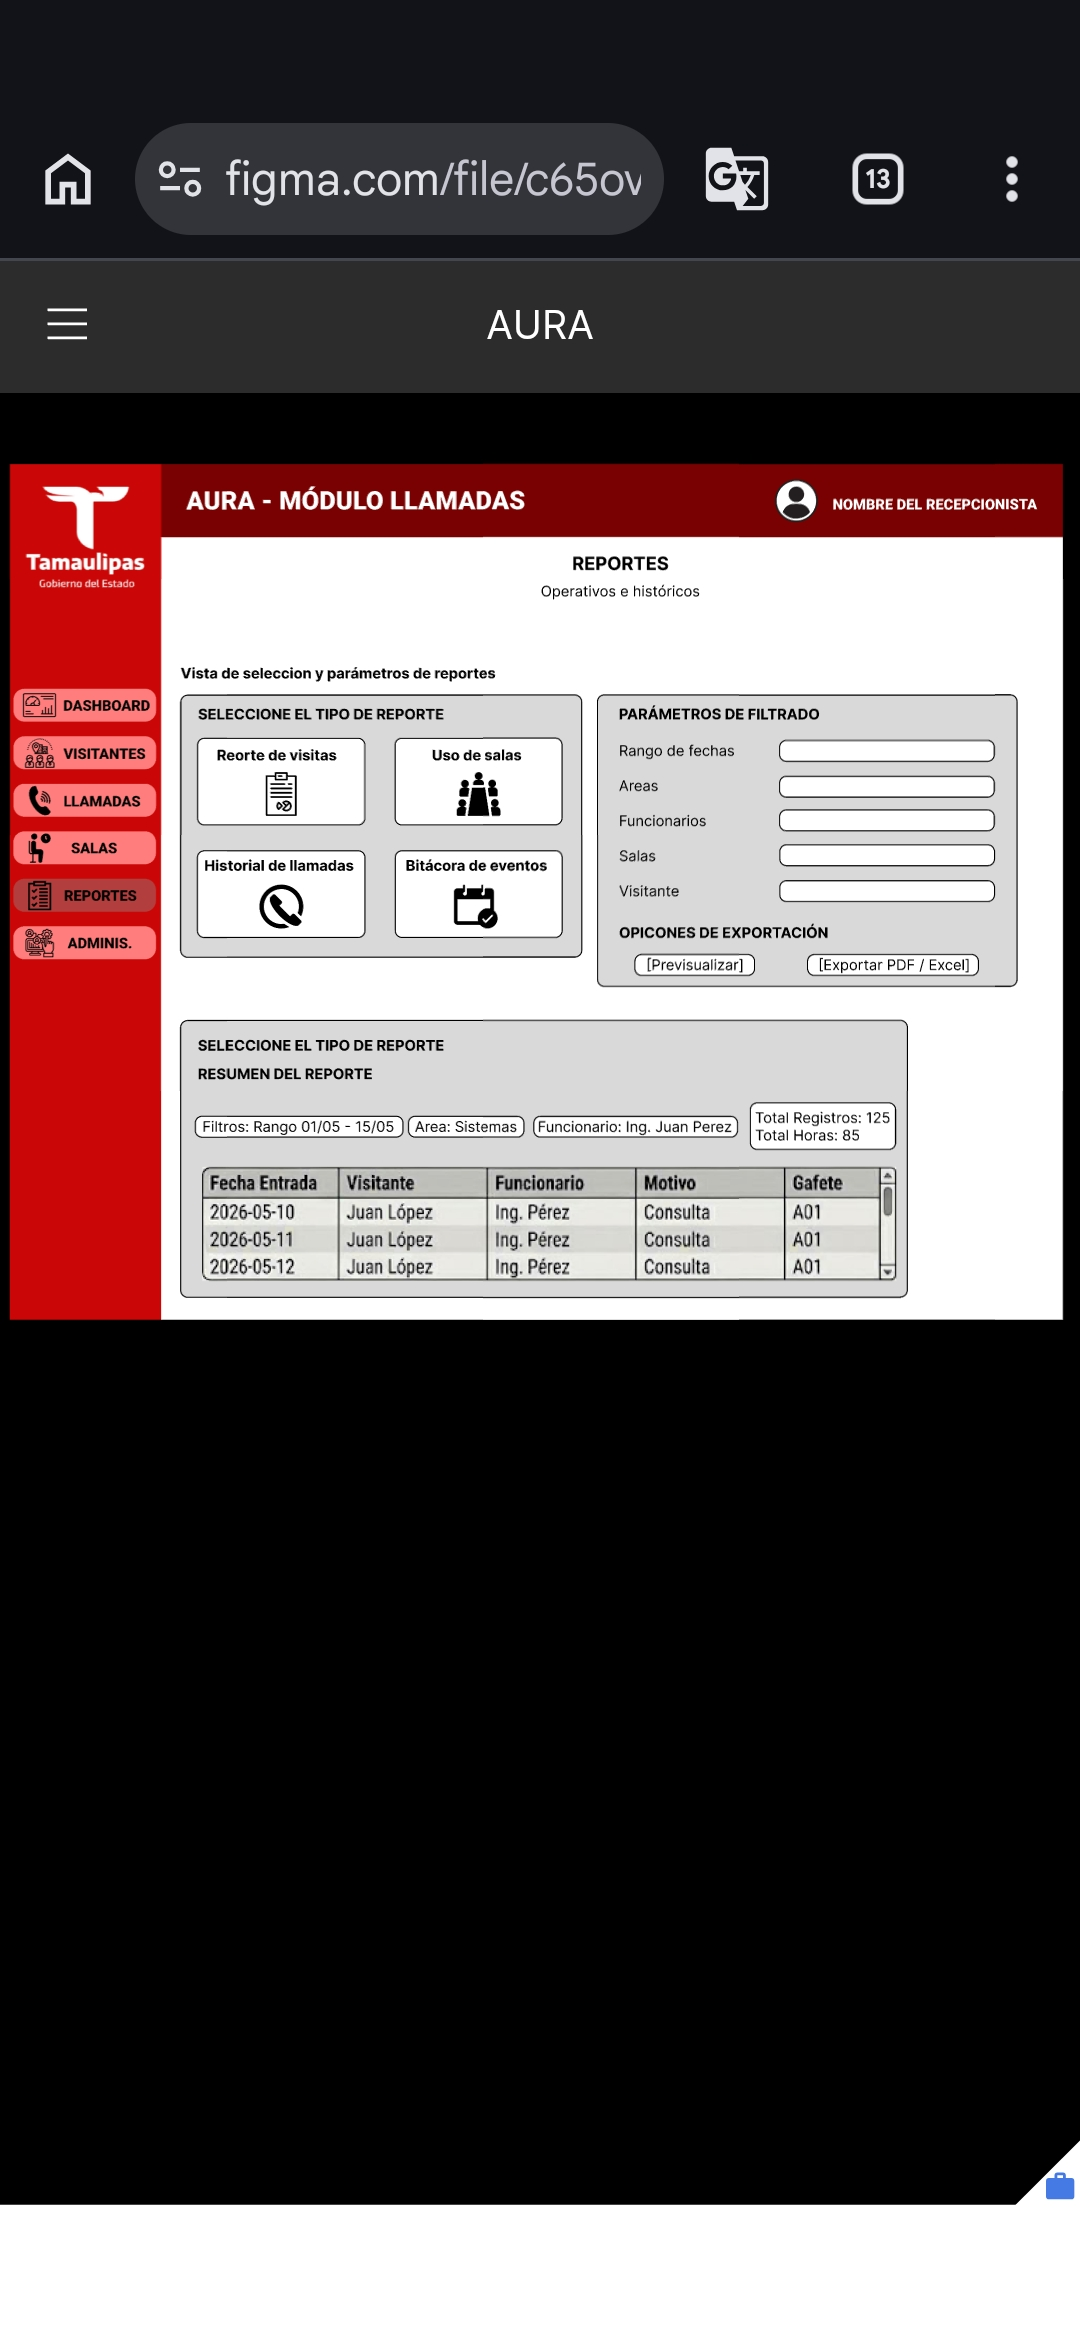
\includegraphics[width=0.4\linewidth]{figs/Reportes.jpg}
    \caption{Modulo de reportes. Diseñado en Figma}
    \label{fig:Reportes}
\end{figure}

\clearpage
\subsection{Construcción de la lógica de negocio y servicios web (APIs) en el Backend con Laravel 13}

Al principio de las estadías, la empresa me compartió un repositorio en donde contendría el starter kit que ellos utilizan para el desarrollo de sus proyectos en Laravel 13. Así que clone el repositorio, lo guarde en mi Terminal de Android y empece con la fase de desarrollo del proyecto en la semana 6.

Durante esa semana, empece a configurar mi terminal Termux de Android para así poder trabajar con Laravel junto con Composer, PostgreSQL, Nodejs-lts y por supuesto, con Git... y seguramente se estará preguntando: ¿Como programaba desde un celular? ¿Como trabajaba con PostgreSQL para la creación de la base de datos, junto con sus tablas y migraciones con Laravel? ¿Como podía levantar el servidor de Laravel desde un celular? 

Son varias preguntas que uno se podría hacer si ve a un desarrollador trabajar desde un móvil, pero tratare de responderlas todas sin mucha drama. Termux en si ya es un entorno aislado y ya viene con el Kernel de Linux instalado, eso quiere decir que podía ejecutar comandos de Linux como si estuviera en una laptop con alguna distro de Linux.. pero claro, Termux tenia su propio gestor de paquetes, por lo que en ves de instalarlos con el típico sudo apt install, lo hacia con pkg install. pkg es el gestor de paquetes de Termux. Asi que si, todo lo que una laptop podría hacer lo podía realizar sin problemas desde mi celular. La única limitante que tuve fue al intentar utilizar Docker, ya que el Kernel de Android no soporta los comandos de Docker... digamos, que es mucho poder para un celular. 

Durante la sexta semana, empece a crear la base de datos Postgres, junto con las tablas correspondientes al proyecto. Por supuesto, si quería que el sistema pudiera reconocer por similitud la fotografía del visitante a la hora de consultarlo, tenia que instalarle la extensión de pgvector a la base de datos. Pgvector permite convertir los datos como texto, imágenes, audios, etc, en vectores numéricos con la finalidad de poder encontrar similitudes a la hora de buscar la fotografía guardada del visitante. En la figura \ref{fig:tablas-BD}, muestro las tablas que contiene el proyecto actualmente.

\begin{figure}[H]
    \centering
    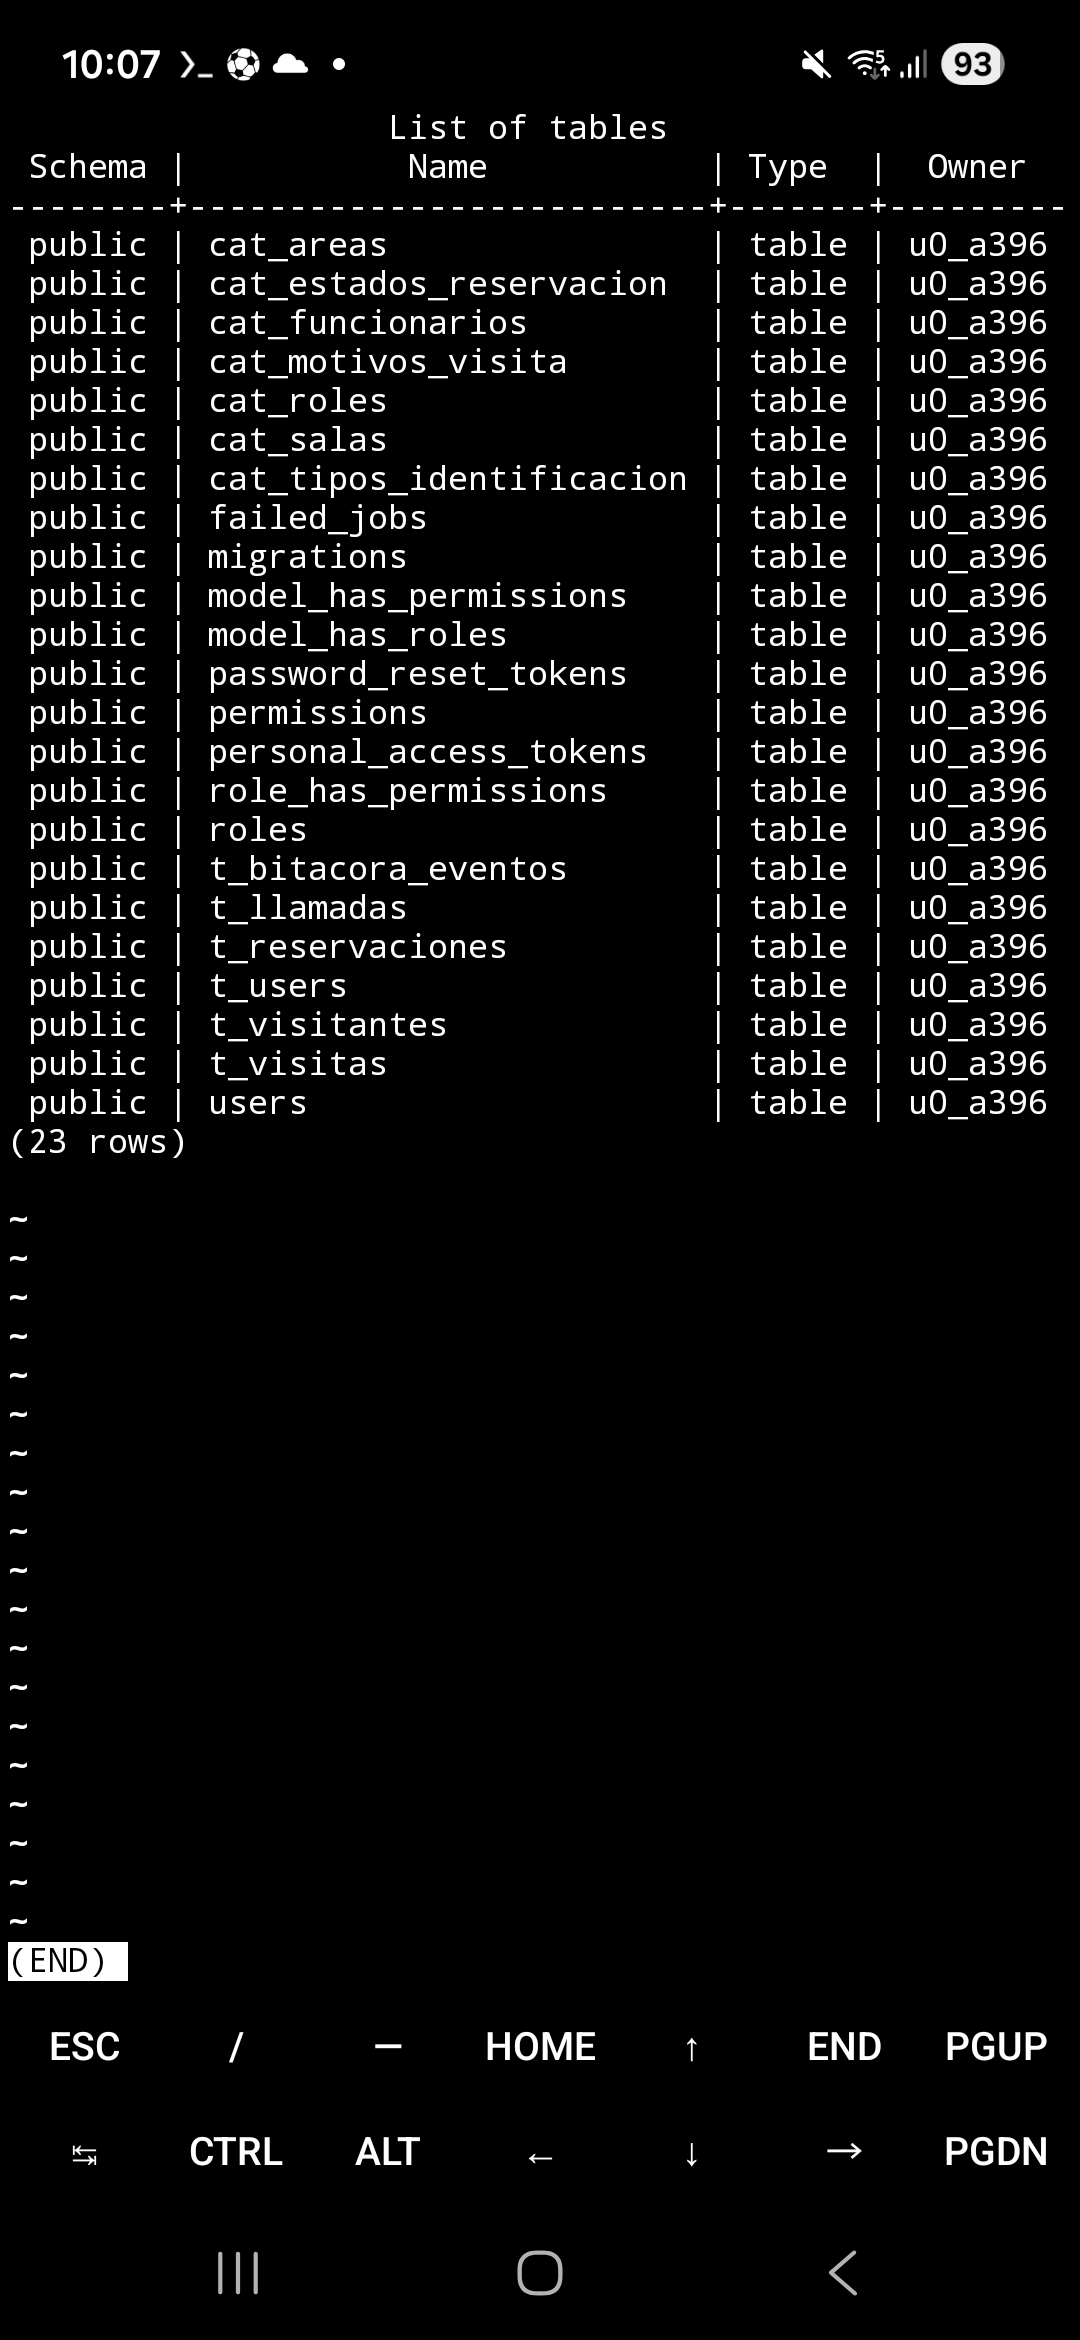
\includegraphics[width=0.5\linewidth]{figs/Tablas-DB.jpg}
    \caption{Tablas de la base de datos del proyecto}
    \label{fig:tablas-BD}
\end{figure}

En esa misma semana, comencé a desarrollar el modulo de Visitantes, que es donde se encontraría la lógica de negocio del registro de visitantes. Ahí mismo cree el controlador, modelos Eloquent para poder comunicarme con las tablas, Request, Actions y Polities. Todo estos componentes tienen un propósito y todos apuntan a la validación de los datos del usuario... es decir, se aseguran de que los datos respeten los tipos de datos de las tablas, que no estén corruptos y que respeten las nomenclaturas definidas en los campos.

En la semana 7, me puse a trabajar en el sistema de autenticación y autorización de los usuarios de la agencia. Para ello, utilice FusionAuth, un servicio externo que lo que hace es redirigir a los usuarios, a un login del propio servicio, para después, otorgarles un token de autorización una vez hayan iniciado sesión en FusionAuth. Después, son llevados nuevamente a la plataforma del proyecto... ya con sus sesiones listas para poder utilizar la plataforma. Todo este protocolo es con la finalidad de que ningún usuario se quiera pasar por un recepcionista o por un administrador de la agencia \cite{AIIDT:accesoTamaulipas}. 

La figura \ref{fig:LoginFusionAuth}, muestra el login de FusionAuth que utiliza el proyecto y la propia Agencia para sus proyectos:

\begin{figure}[H]
    \centering
    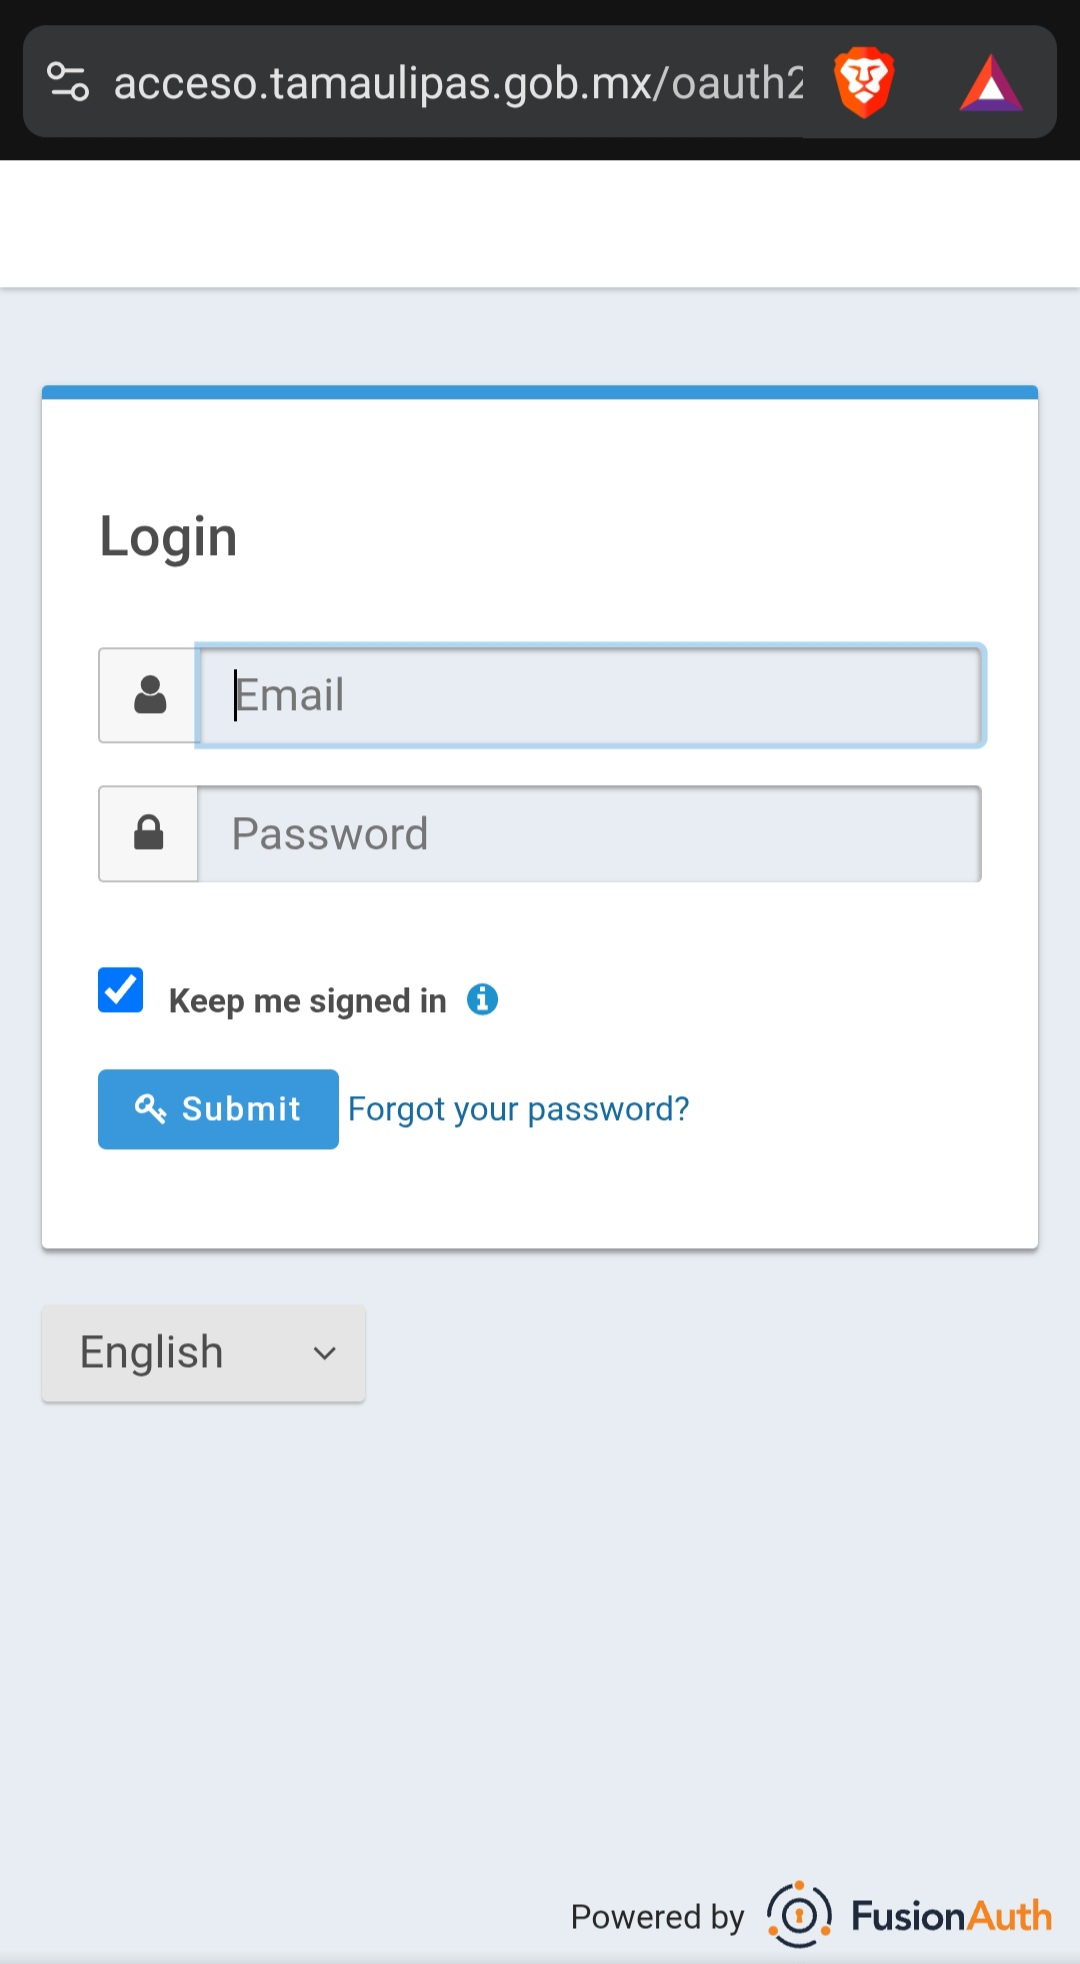
\includegraphics[width=0.4\linewidth]{figs/LoginFusionauth.jpg}
    \caption{Login de FusionAuth que utiliza la Agencia de Innovación e Inteligencia Digital de Tamaulipas}
    \label{fig:LoginFusionAuth}
\end{figure}

Durante esta semana, comencé a pulir las rutas de las API's, como las APIs del registro de visitantes, de visitas, llamadas (las llamadas funcionan como bitácoras) y la de Gestión de salas... pudiendo así integrarlas con éxito a la carpeta de las rutas de Laravel. La figura \ref{fig:RutasAURA}, muestra los endpoints de utiliza el proyecto.

\begin{figure}[H]
    \centering
    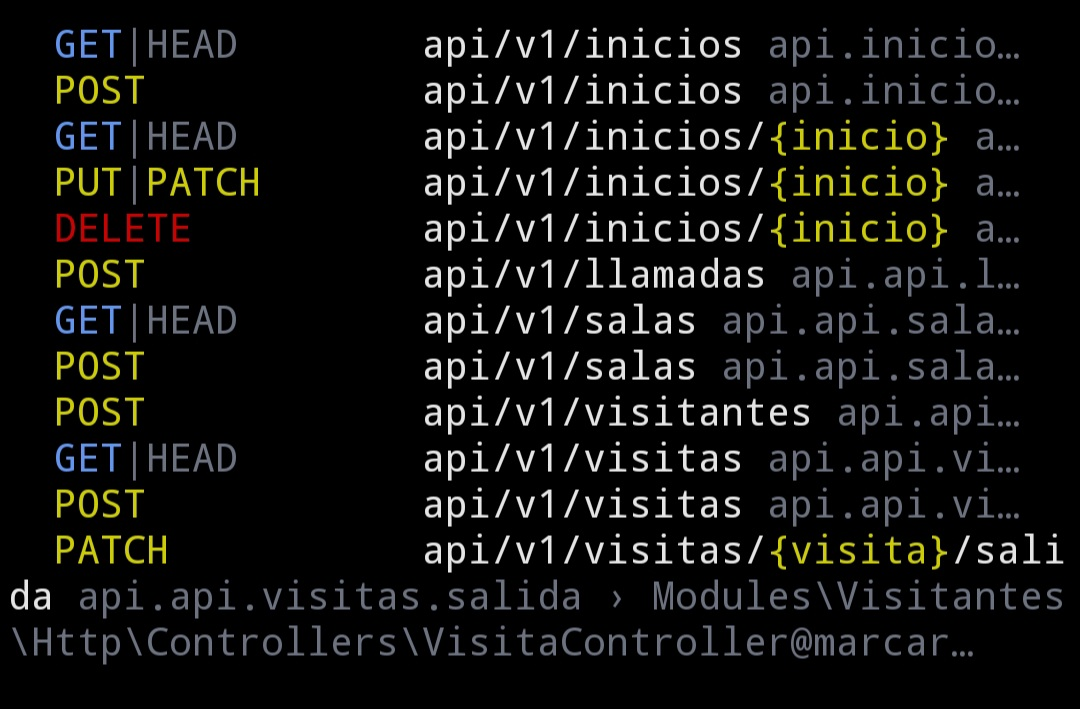
\includegraphics[width=0.4\linewidth]{figs/RutasAURA.jpg}
    \caption{Rutas de las API's del proyecto de estadías en Laravel.}
    \label{fig:RutasAURA}
\end{figure}


\clearpage
\subsection{Desarrollo de interfaces gráficas de usuario basadas en plantillas institucionales}.
La agencia me proporciono códigos HTML sobre los botones, cards y paletas de colores que ellos utilizan para sus proyectos. En la figura \ref{fig:Paleta-colores}, se muestran los códigos fuente que utilizan para la creación de distintos botones.

\begin{figure}[H]
    \centering
    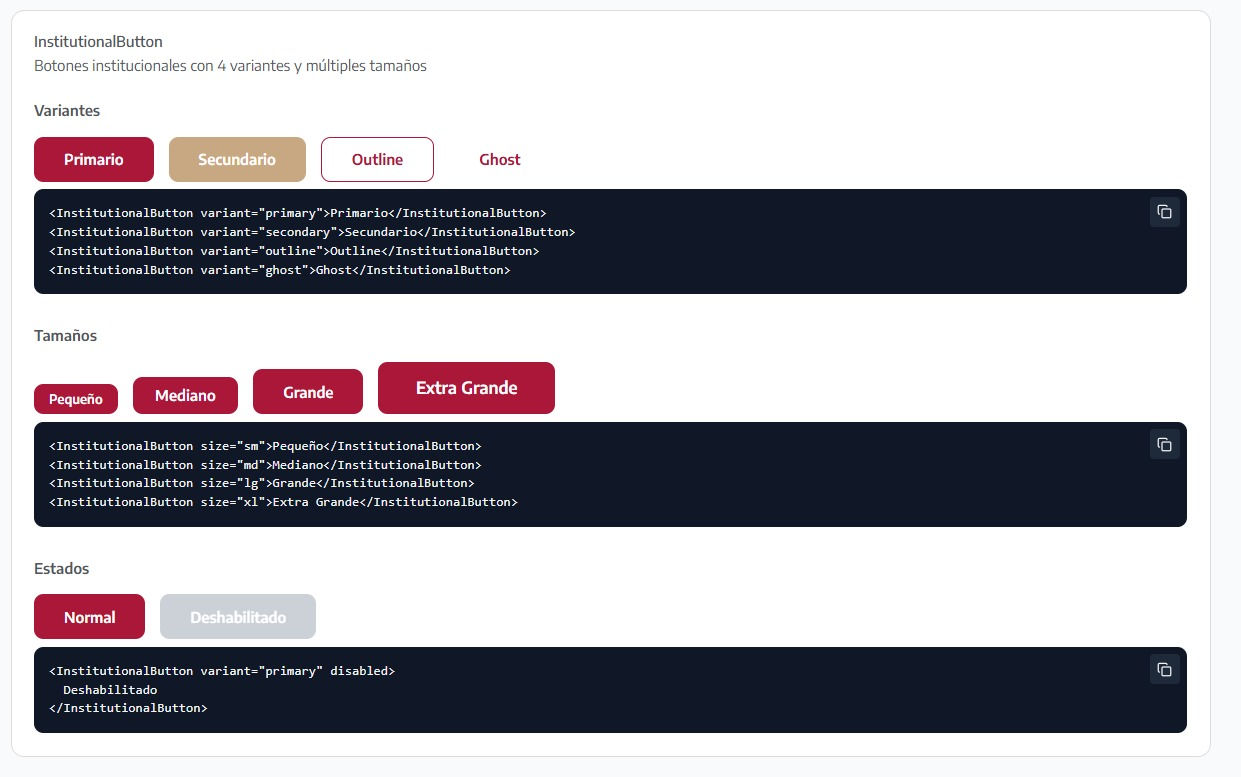
\includegraphics[width=0.7\linewidth]{figs/Paleta-colores.jpg}
    \caption{Diseño de botones que usa la Agencia de Innovación e Inteligencia Digital de Tamaulipas}
    \label{fig:Paleta-colores}
\end{figure}


En la figura \ref{fig:Paleta-colores2}, se muestran los códigos HTML que usan para la creación de distintas tarjetas, con sus respectivos colores.
\begin{figure}[H]
    \centering
    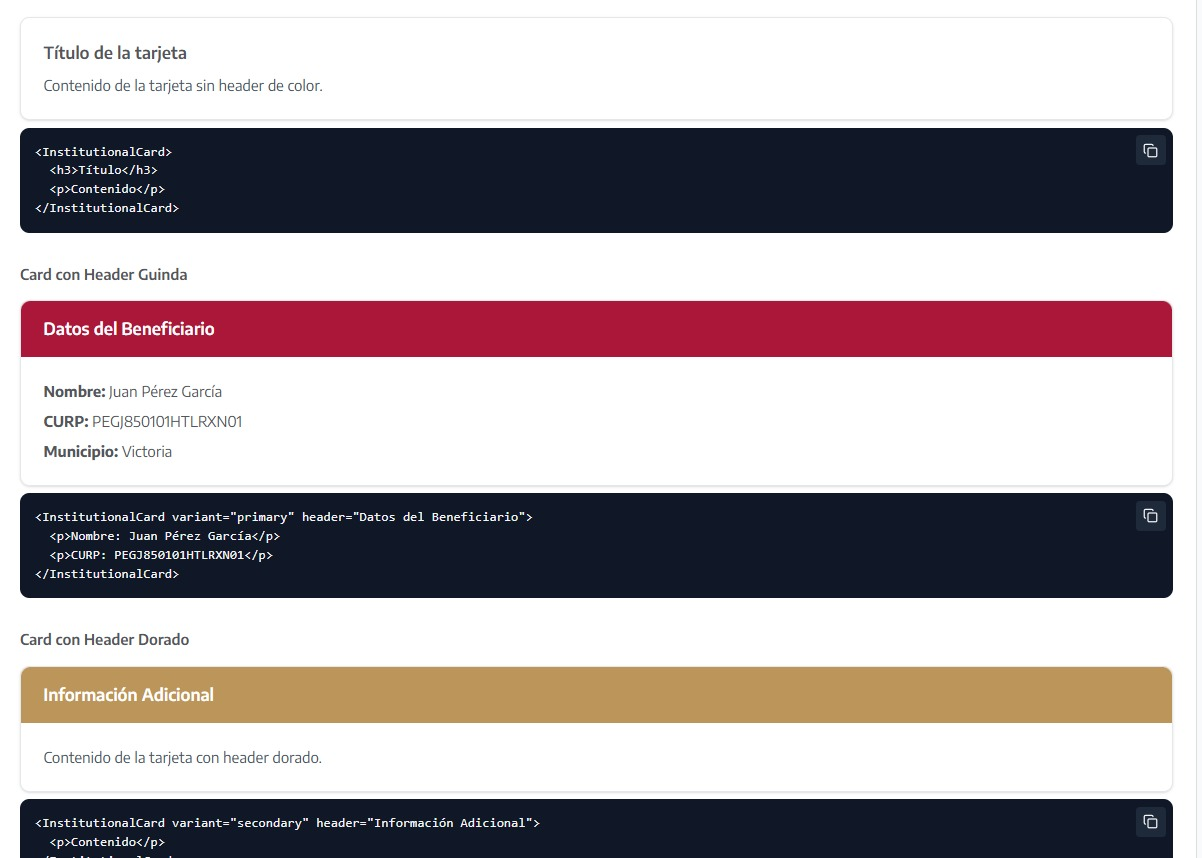
\includegraphics[width=0.7\linewidth]{figs/Paleta-colores2.jpg}
    \caption{Diseño de las tarjetas que usa la Agencia de Innovación e Inteligencia Digital de Tamaulipas}
    \label{fig:Paleta-colores2}
\end{figure}


\clearpage
\subsection{Integración y configuración de algoritmos de identificación biométrica para reconocimiento facial}



\clearpage
\subsection{Ejecución de pruebas de rendimiento, seguridad y consistencia en entornos Docker}



\clearpage
\subsection{Elaboración de documentación técnica, diccionarios de datos y manuales de usuario}




\clearpage
\section{Resultados}




\clearpage
\section{Conclusiones}



%\clearpage
%\section*{Bibliografía}
%Agrega las referencias utilizadas.


\clearpage
%\Urlmuskip=0mu plus 1mu\relax
\addcontentsline{toc}{section}{Bibliografía} 
\printbibliography


\clearpage
\addcontentsline{toc}{section}{Anexos} 


\thispagestyle{fancy}
%\pagenumbering{roman}
%\setcounter{page}{1}
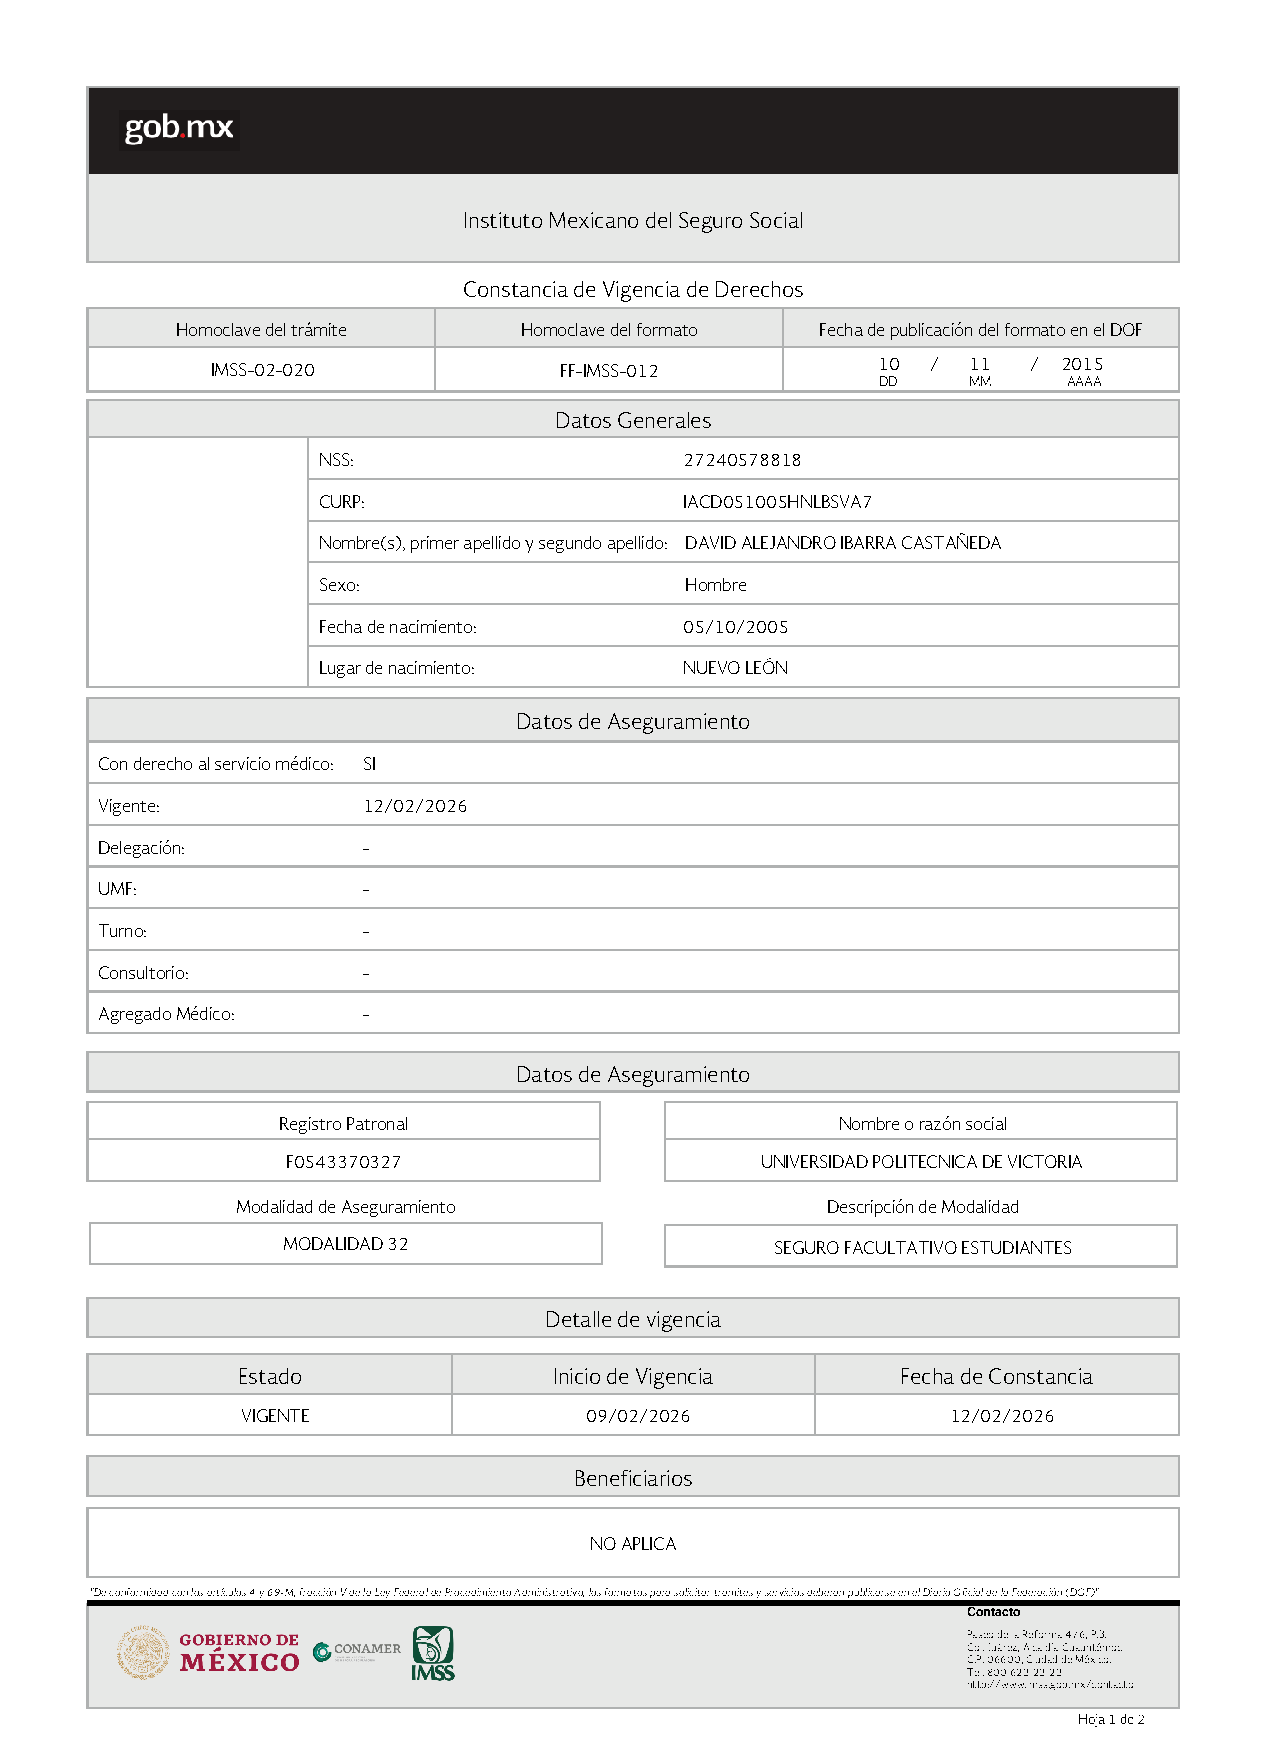
\includepdf[pages={1}]{documentosDigitalizados/SeguroFacultativo.pdf}

% En las siguientes 3 paginas, debe incluir una digitalización de calidad de sus respectivas cartaas, no una fotografia toda cucha tomada con su celular de Coppel
% Pagina 1: Digitalización de la carta de presentación (sustituir por una original en el empastado)
\clearpage
\thispagestyle{fancy}
%\pagenumbering{roman}
%\setcounter{page}{1}

\includepdf[pages={1}]{documentosDigitalizados/CartaPresentacion.pdf}

% Pagina 2: Digitalización de la carta de aceptación (sustituir por una original en el empastado)

\clearpage
\thispagestyle{fancy}
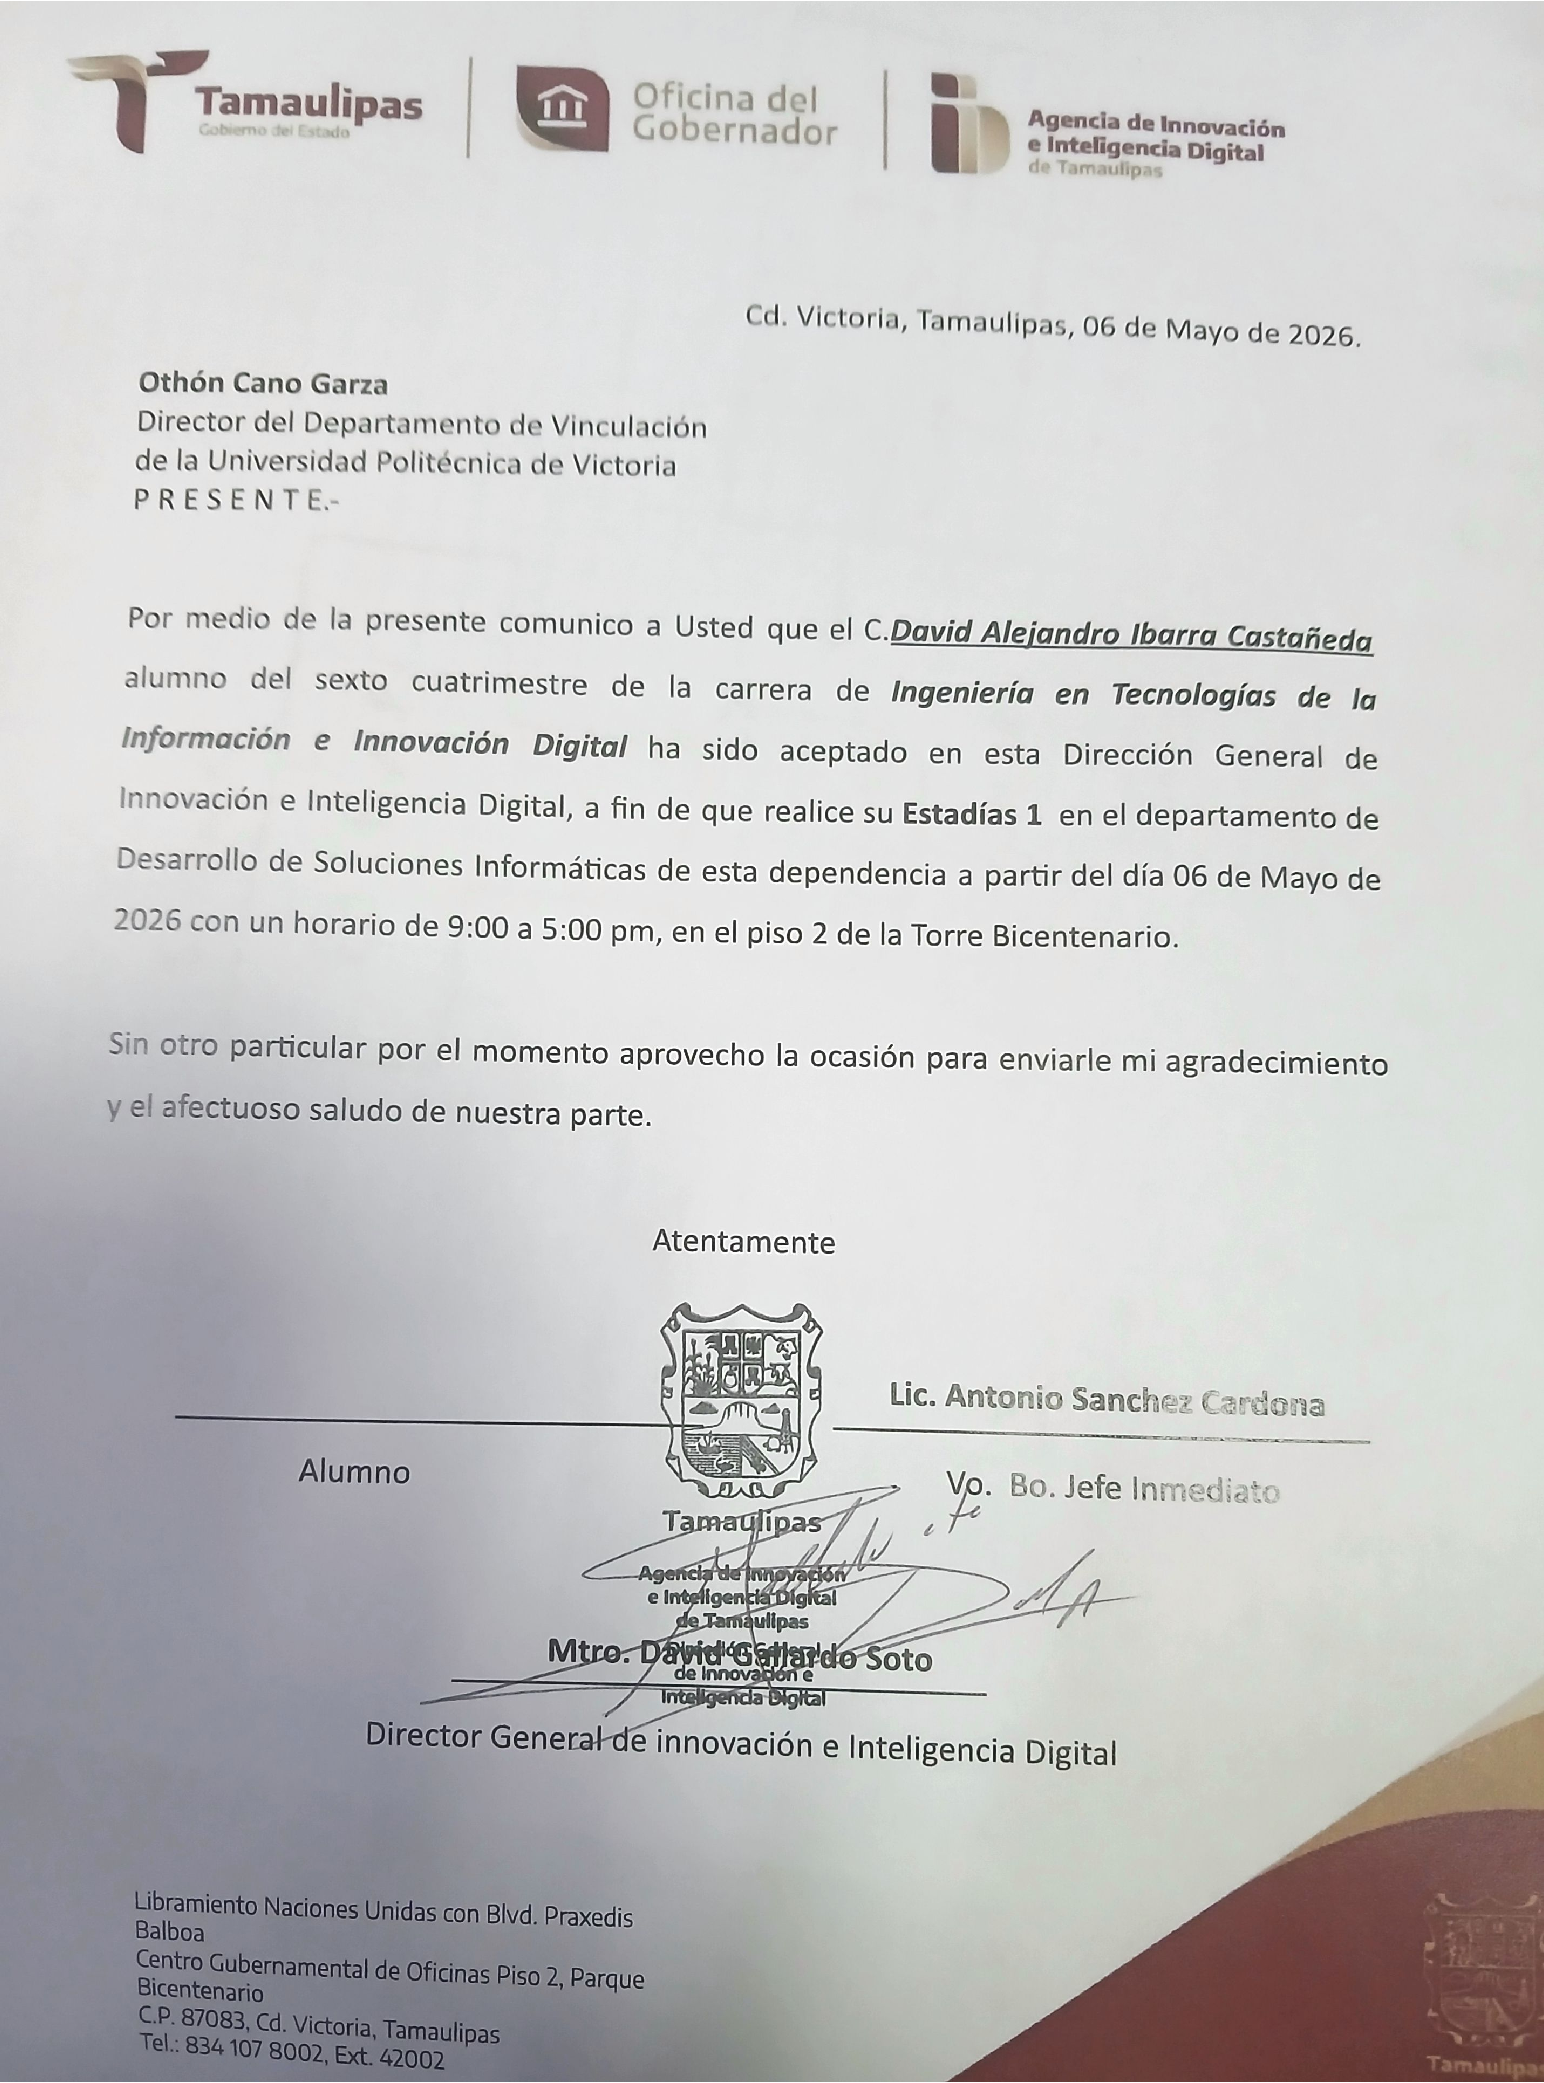
\includepdf[pages={1}]{documentosDigitalizados/CartaAceptacion.pdf}

% Pagina 3: Digitalización de la carta de liberación (sustituir por una original en el empastado)

%\clearpage
%\thispagestyle{fancy}
%
\includepdf[pages={1}]{documentosDigitalizados/CartaLiberacion.pdf}

%\chapter*{Rúbrica para la Evaluación del Reporte de Estadía}
\clearpage
%\section*{Rúbrica para la Evaluación del Reporte de Estadía}
\newcommand{\SizeFont}{\footnotesize}

\begin{center}
\large {\textbf{Rúbrica para la Evaluación del Reporte de Estadía}}
\end{center}

\begin{longtable}{|C{1cm}|C{9cm}|C{2cm}|C{3cm}|}
\hline
%Fecha y lugar en que se emite: \textbf{Ciudad Victoria, Tamaulipas, a \fechaAutorizacionInforme } \\[0.125cm]
\multicolumn{4}{|l|}{Nombre completo del estudiante: \textbf{\NombreAlumno} }\\
\multicolumn{4}{|l|}{Matrícula:  \textbf{\Matricula}}  \\
\multicolumn{4}{|l|}{PERIODO: \ncuatrimestre } \\
\multicolumn{4}{|l|}{Nombre del evaluador: \nasesorinstitucional} \\
\multicolumn{4}{|l|}{ } \\
\multicolumn{4}{|l|}{Firma del Evaluador: \_\_\_\_\_\_\_\_\_\_\_\_\_\_\_\_\_\_\_\_\_\_\_\_  }\\
\multicolumn{4}{|l|}{Calificación Final: \_\_\_ / 100} \\ \hline
Valor & Características a cumplir & Puntos & Observaciones \\ \hline
\SizeFont 6 & \SizeFont Resumen ejecutivo y abstract: Indica qué se realizó, cómo se realizó y qué se obtuvo. (una cuartilla en español e inglés) & & \\ \hline
\SizeFont 6 & \SizeFont Contenido temático: Describe correctamente el contenido del documento & & \\ \hline
\SizeFont 6 & \SizeFont Introducción: El informe cumple con introducir al lector de una manera atractiva el panorama general del trabajo realizado en la unidad económica.  & & \\ \hline
\SizeFont 6 & \SizeFont Descripción de la unidad económica: Se redactan los detalles de los antecedentes del departamento, la empresa, giro, misión, visión, infraestructura, ubicación. & & \\\hline
\SizeFont 6 & \SizeFont Objetivos operativos: Describen las acciones a cumplir mediante actividades establecidas por el asesor empresarial & & \\ \hline
\SizeFont 24 & \SizeFont Metodología: Descripción a detalle de las etapas y procedimientos utilizados en el proyecto & & \\ \hline
\SizeFont 18 & \SizeFont Resultados: Interpreta y analiza los resultados obtenidos durante su estadía. & & \\ \hline
\SizeFont 12 & \SizeFont Conclusiones: Las conclusiones son claras y acordes con el objetivo esperado & & \\ \hline
\SizeFont 6 & \SizeFont Bibliografía y anexos: Cita correctamente las fuentes de información utilizando un estilo de referencia; anexa cartas correspondientes & & \\ \hline
\SizeFont 10 & \SizeFont Responsabilidad: Entregó el reporte en la fecha y hora señalada. Asistió al menos al 80\% de sus días de Estadía & & \\ \hline
\end{longtable}

%\chapter*{Rúbrica para Exposición}
\clearpage
\begin{center}
\large {\textbf{Rúbrica para Exposición del Reporte de Estadía}}
\end{center}


\begin{longtable}{|p{3.75cm}|p{3.75cm}|p{3.75cm}|p{3.75cm}|}
\hline
 & \multicolumn{3}{c|}{Nivel de logro} \\ \hline
%A &B  & C & D \\
Criterio &  Bueno ( 10\% ) & Regular (7\% ) & Menor a lo esperado (5\%) \\ \hline
\SizeFont Dominio del tema (10\%) & \SizeFont Utiliza todos los términos y conceptos de manera correcta. & \SizeFont Utiliza la mayoría términos y conceptos de manera correcta & \SizeFont Confunde los términos y conceptos. \\ \hline

\SizeFont  Presentación de material visual (10\%) & \SizeFont Las  diapositivas usadas tienen fondo claro, letras, tablas e imágenes visibles. La presentación contiene los aspectos relevantes de la Estadía
& \SizeFont Las  diapositivas usadas presentan dificultad para su apreciación visual. La presentación contiene los aspectos relevantes de la Estadía & \SizeFont Las  diapositivas usadas presentan dificultad para su apreciación visual. La presentación carece de algunos aspectos relevantes de la Estadía. \\ \hline

\SizeFont   Comunicación y expresión (10\%)  & \SizeFont   Su volumen de voz es comprensible. Su expresión corporal manifiesta seguridad ejecutiva. Su atuendo cumple los estándares de ser formal o semiformal.  Mantiene una línea de respeto en general. &  \SizeFont   Su volumen de voz no es comprensible. Su expresión corporal manifiesta inseguridad. Su atuendo cumple los estándares de ser formal o semiformal.  Mantiene una línea de respeto en general. &
\SizeFont  Su volumen de voz no es comprensible. Su expresión corporal manifiesta inseguridad. Su atuendo no cumple los estándares de ser formal o semiformal.  Realiza alguna falta de respeto. \\ \hline

\SizeFont   Respuestas (10\%) & \SizeFont Las respuestas son consistentes y con parámetros de lógica operativa. & \SizeFont    Las respuestas no son consistentes pero tienen parámetros de lógica operativa. & \SizeFont    Las respuestas son difusas e incoherentes.  \\ \hline


\multicolumn{2}{|c|}{\textbf{Ponderación final de su exposición:}} & \multicolumn{2}{c|}{\_\_\_ /100} \\ \hline
%\multicolumn{2}{|c|}{Día / Mes / Año} &  \multicolumn{2}{c|}{\_\_\_\_ / \_\_\_\_\_\_\_\_ / \_\_\_\_  } \\  \hline
\multicolumn{2}{|c|}{Día / Mes / Año} &  \multicolumn{2}{c|}{\DiaEvaluacionPesentacion / \MesEvaluacionPesentacion / \AnhoEvaluacionPesentacion} \\  \hline
\multicolumn{2}{|c}{ }& \multicolumn{2}{|c|}{ }  \\
\multicolumn{2}{|c}{ }& \multicolumn{2}{|c|}{ }  \\    
\multicolumn{2}{|c}{Comentario adicional} & \multicolumn{2}{|c|}{ } \\  
\multicolumn{2}{|c}{ }& \multicolumn{2}{|c|}{ }  \\  
\multicolumn{2}{|c}{ }& \multicolumn{2}{|c|}{ }  \\  \hline



\end{longtable}

\end{document}








\end{document}
%\section*{Rúbrica para Exposición}
%Completa aquí los criterios de dominio del tema, material visual, comunicación y respuestas.

%\usepackage{longtable}
%\usepackage{array}

\begin{center}
\textbf{RÚBRICA PARA LA EVALUACIÓN DEL REPORTE DE ESTADÍA}
\end{center}

\vspace{0.5cm}

\noindent
\textbf{NOMBRE DEL ESTUDIANTE:} NOMBRES Y APELLIDOS

\noindent
\textbf{PERIODO:} MAYO AGOSTO 2026

\noindent
\textbf{NOMBRE DEL EVALUADOR:} NOMBRES Y APELLIDOS

\noindent
\textbf{FIRMA DEL EVALUADOR:}

\noindent
\textbf{CALIFICACIÓN FINAL:} 60/100

\vspace{0.5cm}

\begin{longtable}{|c|C{7cm}|c|C{4cm}|}
\hline
\textbf{Valor} & \textbf{Características a cumplir} & \textbf{Puntos obtenidos} & \textbf{Observaciones} \\
\hline
6 & Resumen ejecutivo y abstract: Indica qué se realizó, cómo se realizó y qué se obtuvo. (una cuartilla en español e inglés) & & \\
\hline
6 & Contenido temático: Describe correctamente el contenido del documento & & \\
\hline
6 & Introducción: El informe cumple con introducir al lector de una manera atractiva el panorama general del trabajo realizado en la unidad económica. & & \\
\hline
6 & Descripción de la unidad económica: Se redactan los detalles de los antecedentes del departamento, la empresa, giro, misión, visión, infraestructura, ubicación. & & \\
\hline
6 & Objetivos operativos: Describen las acciones a cumplir mediante actividades establecidas por el asesor empresarial & & \\
\hline
24 & Metodología: Descripción a detalle de las etapas y procedimientos utilizados en el proyecto & & \\
\hline
18 & Resultados: Interpreta y analiza los resultados obtenidos durante su estadía. & & \\
\hline
12 & Conclusiones: Las conclusiones son claras y acordes con el objetivo esperado & & \\
\hline
6 & Bibliografía y anexos: Cita correctamente las fuentes de información utilizando un estilo de referencia; anexa cartas correspondientes & & \\
\hline
10 & Responsabilidad: Entregó el reporte en la fecha y hora señalada. Asistió al menos al 80\% de sus días de Estadía & & \\
\hline
\end{longtable}

%\vspace{1cm}

\clearpage
\begin{center}
\textbf{RÚBRICA PARA EXPOSICIÓN DEL REPORTE DE ESTADÍAS}
\end{center}

\begin{center}
\textbf{Técnico Superior Universitario}
\end{center}

\vspace{0.5cm}
\newcommand{\SizeFont}{\small}
\begin{longtable}{|p{3cm}|p{4cm}|p{4cm}|p{4cm}|}
\hline
\textbf{Criterio} & \textbf{Bueno (10\%)} & \textbf{Regular (7\%)} & \textbf{Menor a lo esperado (5\%)} \\
\hline
Dominio del tema & Utiliza todos los términos y conceptos de manera correcta. & Utiliza la mayoría de los términos y conceptos de manera correcta. & Confunde los términos y conceptos. \\
\hline
Presentación de material visual & Las diapositivas tienen fondo claro, con elementos visibles y contienen aspectos relevantes. & Presentan dificultad visual pero incluyen aspectos relevantes. & Presentan dificultad visual y carecen de aspectos relevantes. \\
\hline
Comunicación y expresión & Voz comprensible, seguridad corporal, atuendo formal o semiformal y respeto. & Voz poco comprensible, inseguridad, pero mantiene formalidad. & Voz no comprensible, inseguridad, atuendo inadecuado o falta de respeto. \\
\hline
Respuestas & Respuestas consistentes con lógica operativa. & Respuestas poco consistentes pero con lógica. & Respuestas difusas e incoherentes. \\
\hline
\end{longtable}

\vspace{0.5cm}

\noindent
\textbf{Ponderación final de su exposición:} 40/100

\vspace{0.5cm}

\noindent
\textbf{Datos de la exposición y evaluación}

\noindent
Día / Mes / Año

\noindent
Comentario adicional

\vspace{1cm}

\noindent
Firma \hspace{3cm} Nombre \hspace{3cm} Correo electrónico

\vspace{0.5cm}

\noindent
Profesor asesor institucional

\end{document}
